 % ============================================================
%  KOS Course Project Report — Group B (Lamia)
%  Natural Language <-> SPARQL Translation System
%  University of Geneva, MSc in Digital Systems and Services
% ============================================================

\documentclass[11pt,a4paper]{article}

% --------------- Encoding & language ------------------------
\usepackage[utf8]{inputenc}    % UTF-8 source encoding
\usepackage[T1]{fontenc}       % Better font encoding (accents, etc.)
\usepackage[english]{babel}    % English typesetting rules

% --------------- Page geometry & typography -----------------
\usepackage[a4paper,margin=2.5cm]{geometry}  % Page margins
\usepackage{microtype}                       % Subtle typography improvements
\usepackage{setspace}     
\onehalfspacing                              % 1.5 line spacing
\usepackage{parskip}                         % Paragraph spacing instead of indent

% --------------- Maths & symbols ----------------------------
\usepackage{amsmath,amssymb,amsthm}      
% \usepackage{siunitx}                       % Numbers, units, alignment (not used)

% --------------- Figures, tables, captions ------------------
\usepackage{graphicx}                        % Include images
\graphicspath{{figures/}}                    % Default folder for figures
\usepackage{caption}          
\usepackage{subcaption}                      % Sub-figures
\usepackage{booktabs}                        % \toprule, \midrule, \bottomrule
\usepackage{tabularx}                        % Flexible tables
% \usepackage{multirow}                      % Not used in this document
\usepackage{float}                           % [H] placement for figures/tables

% --------------- Lists --------------------------------------
\usepackage{enumitem}                        % Compact, customisable lists
\setlist{itemsep=2pt, topsep=4pt}            % Tighter default spacing

% --------------- Colours ------------------------------------
\usepackage{xcolor}
\usepackage{pifont}
\newcommand{\cmark}{\ding{51}}%
\newcommand{\xmark}{\ding{55}}%
\definecolor{accentpurple}{HTML}{7C5CFC}     % Matches the UI accent colour
\definecolor{codebg}{HTML}{F5F2FF}           % Light purple code background
\definecolor{codeborder}{HTML}{C4B8E0}
\definecolor{codekw}{HTML}{5A3ED4}           % SPARQL keywords
\definecolor{codestr}{HTML}{0E7490}          % Strings
\definecolor{codecomment}{HTML}{6B6080}      % Comments
\definecolor{codevar}{HTML}{B45309}          % SPARQL variables (?x)

% --------------- Source code listings -----------------------
\usepackage{listings}

% Generic listing style
\lstdefinestyle{baseStyle}{
    backgroundcolor=\color{codebg},
    rulecolor=\color{codeborder},
    frame=single,
    framerule=0.4pt,
    basicstyle=\ttfamily\footnotesize,
    keywordstyle=\color{codekw}\bfseries,
    stringstyle=\color{codestr},
    commentstyle=\color{codecomment}\itshape,
    breaklines=true,
    breakatwhitespace=true,
    columns=fullflexible,
    keepspaces=true,
    showstringspaces=false,
    captionpos=b,
    xleftmargin=8pt,
    xrightmargin=4pt,
    aboveskip=8pt,
    belowskip=8pt,
}

% Custom SPARQL style
\lstdefinelanguage{SPARQL}{
    morekeywords={SELECT, DISTINCT, REDUCED, WHERE, FILTER, FROM, OPTIONAL,
                  UNION, GRAPH, ORDER, BY, LIMIT, OFFSET, GROUP, HAVING,
                  ASK, CONSTRUCT, DESCRIBE, PREFIX, BASE, SERVICE, BIND,
                  AS, MINUS, NOT, EXISTS, IN, LANG, STR, REGEX, COUNT,
                  SUM, MIN, MAX, AVG, ASC, DESC, a},
    morestring=[b]",
    morecomment=[l]{\#},
    sensitive=true,
    alsoletter={?},
}

% Style for SPARQL listings
\lstdefinestyle{sparqlStyle}{
    style=baseStyle,
    language=SPARQL,
}

% Style for Python listings
\lstdefinestyle{pythonStyle}{
    style=baseStyle,
    language=Python,
}

% Style for plain text / YAML / JSON-ish listings
\lstdefinestyle{plainStyle}{
    style=baseStyle,
    language=,
}

% --------------- Hyperlinks & cross-references --------------
\usepackage{url}                
\usepackage[colorlinks=true,
            linkcolor=accentpurple,
            citecolor=accentpurple,
            urlcolor=accentpurple]{hyperref} % Coloured PDF links
\usepackage{cleveref}                        % \cref{...} smart references (must be loaded AFTER hyperref)

% --------------- Bibliography -------------------------------
\usepackage[numbers,sort&compress]{natbib}

% --------------- "TODO" macro for drafting ------------------
\newcommand{\todo}[1]{\textcolor{red}{\textbf{[TODO: #1]}}}

% ============================================================
%                       DOCUMENT BEGINS
% ============================================================
\begin{document}

% --------------- Title metadata -----------------------------
\begin{titlepage}
    \centering

    \vspace*{2.2cm}

    {\Huge\bfseries
    Bidirectional Translation Between Natural Language and SPARQL
    \par}

    \vspace{0.8cm}

    {\large
    \begin{tabular}{ccc}
        Engin Samet Dede & Sevgi Dilay Demirci & Kamar El Morabit \\[0.6em]
        Jumainah Khan    & Saïfudeen Hisham Kolikara Mahin
    \end{tabular}
    \par}

    \vspace{2cm}

    {\large Group B (Lamia)\par}

    \vspace{0.4cm}

    {\normalsize
    University of Geneva\\[0.25em]
    Course: Knowledge Organization Systems
    \par}

    \vfill
\end{titlepage}

% ------------------------------------------------------------
% ABSTRACT
% ------------------------------------------------------------
\begin{abstract}
\noindent
This project presents a bidirectional Natural Language and SPARQL translation system designed to make large public knowledge graphs easier to access. The system allows users to ask questions in ordinary English and automatically generates SPARQL queries for Wikidata or DBpedia. It also supports the reverse direction by explaining existing SPARQL queries in natural language, helping users understand what a query is doing before or after execution.

The prototype is built around a Streamlit interface, domain specific YAML configuration files, and large language models accessed through Hactar and Hugging Face. The main design choice is to guide the models with endpoint-specific prefixes, ontology hints, and few-shot examples rather than fine tuning them. This makes the system easier to extend to new domains while keeping the query generation process transparent.

The project also includes query cleaning, retry mechanisms, result summarisation, knowledge graph visualisation, and an evaluation framework for comparing models across multiple domains. The evaluation shows that both Qwen and Llama can often generate executable and semantically meaningful SPARQL queries, but failures still occur because of hallucinated identifiers, endpoint timeouts, schema mismatches, and noisy knowledge graph data. Overall, the project demonstrates that LLM based SPARQL generation is useful for lowering the access barrier to knowledge graphs, but it still requires careful domain configuration, deterministic post-processing, and transparent evaluation.
\end{abstract}

\clearpage
\tableofcontents
\newpage

% ============================================================
\section{Introduction}
\label{sec:intro}
% Suggested length: ~800-1000 words.
% Goals of this section:
%   - Motivate why NL <-> SPARQL matters in the KOS context.
%   - State the problem clearly.
%   - Summarise what was built and the contributions.
%   - Give the reader a roadmap of the paper.
% ============================================================

% ---- 1.1 Motivation / Context -------------------------------
\subsection{Motivation and Problem Statement }
\label{sec:motivation}

Large public knowledge graphs such as Wikidata and DBpedia contain a huge amount of structured information on many variety of domains. In theory, this information is openly accessible. In practice, however, accessing it is not simple for most users, because the information has to be retrieved through SPARQL queries.

Writing SPARQL requires more than just knowing what question to ask. The user also needs to know the syntax of the query language, the correct endpoint, the relevant prefixes, and the specific classes and properties used by each knowledge graph. For a non-technical user, this creates a clear barrier: the knowledge is available, but it is difficult to reach.

This project addresses that problem by building a system that translates between natural language and SPARQL. In the natural language to SPARQL direction, the user asks a question in ordinary English, and the system generates a query for the selected knowledge graph. In the SPARQL to natural language direction, the system explains an existing query in a more readable form, helping the user understand what the query is doing. Since it is possible that a small mistake can lead to an invalid query, an empty result, or a correct-looking query that answers the wrong question, much of the project focuses on domain specific prompting, query cleaning, execution, and evaluation.

\paragraph{Contributions.}
The main contributions of this project are: (i) a working bidirectional NL$\leftrightarrow$SPARQL prototype covering ten domains across Wikidata and DBpedia; (ii) a two-phase entity and predicate resolution step that replaces static, hand-curated identifiers with API-backed lookups at query time; (iii) a per-domain YAML configuration system that extends to new domains without code changes; (iv) a multi-model arena with structured user feedback and a composite evaluation framework that combines structural metrics with an LLM-as-a-Judge layer.

\paragraph{Paper organisation.}
Section~\ref{sec:background} covers the technical background on knowledge graphs, SPARQL, and language models. Section~\ref{sec:system} describes the overall architecture and user interface. Section~\ref{sec:methodology} details the core design choices. Section~\ref{sec:implementation} covers the technology stack and practical engineering issues encountered. Section~\ref{sec:evaluation} presents the evaluation setup, results, and qualitative analysis. Section~\ref{sec:discussion} discusses limitations and future directions, and Section~\ref{sec:conclusion} concludes.

% ============================================================
\section{Background}
\label{sec:background}
% Suggested length: ~1200-1400 words.
% Subsections give a clean structure. Each subsection should
% finish with ONE sentence linking back to the project.
% ============================================================

\subsection{Knowledge Organization Systems}
\label{sec:kos}

Knowledge organization systems (KOS) range from simple term lists and thesauri at one end to formal ontologies at the other, with the key difference being how explicitly semantic relationships are defined \cite{hodge2000kos,zeng2008kos}. Wikidata and DBpedia sit at the formal end of that spectrum. Both use globally unique URIs for entities, define properties with domains and ranges, and organise data into class hierarchies that can be queried formally \cite{vrandecic2014wikidata,lehmann2015dbpedia}.

The practical consequence is that these knowledge bases are machine-readable but not directly accessible to users without training. Retrieving information requires knowing SPARQL, the local property naming conventions, and enough of the data model to write structurally correct queries. Making that access easier is the core motivation for this project. The two graphs also differ from each other in ways that matter technically: Wikidata identifies everything with opaque Q-IDs and P-IDs, while DBpedia uses readable names like \texttt{dbo:director}, so any system that supports both has to manage two different vocabularies and two different endpoint behaviours.

\subsection{The Semantic Web Stack and Linked Data}
\label{sec:linkeddata}

The Semantic Web is built on a layered set of standards. RDF (Resource Description Framework) is the base layer: it represents any statement as a subject-predicate-object triple, where each element is either a URI or a literal. Because URIs are globally unique, RDF datasets from different sources can be combined without any schema-matching step. RDFS and OWL build on top of RDF to add class hierarchies, property constraints, and logical axioms, making it possible to define and reason over formal ontologies.

Bizer, Heath, and Berners-Lee formalised how to publish and interconnect RDF data through four Linked Data principles: name things with URIs, make those URIs look-up\-able over HTTP, return RDF when they are looked up, and include links to related URIs \cite{bizer2009linkeddata}. Wikidata and DBpedia are among the most central nodes in the Linked Open Data cloud that these principles created. Both expose public SPARQL endpoints, which is where this project connects to the stack. SPARQL queries a graph by describing a pattern of triples to match against the stored data \cite{w3c2013sparql}. It is powerful enough to express complex questions, but it requires the user to know the structure of the target graph in detail. That gap between what a user wants to ask and what SPARQL needs to execute is exactly what this project addresses.

\subsection{SPARQL}
\label{sec:sparql}

SPARQL is the standard query language for RDF graphs, standardised by
the W3C \cite{w3c2013sparql}. Where SQL queries tables, SPARQL queries
a graph of triples by describing a pattern of triples to match. A
query is built from a basic graph pattern, a set of triple
patterns in which any of the subject, predicate, or object positions
can be a variable. The query engine finds every subgraph of the data
that matches the pattern and binds the variables accordingly.

A query uses one of four forms. \texttt{SELECT} returns a table of
variable bindings, \texttt{ASK} returns a boolean, \texttt{CONSTRUCT}
builds a new RDF graph from the matches, and \texttt{DESCRIBE} returns
RDF about a resource. On top of basic graph patterns, SPARQL adds
\texttt{FILTER} for value constraints, \texttt{OPTIONAL} for matches
that may or may not be present, \texttt{UNION} for alternatives, and
aggregation with \texttt{GROUP BY}. These constructs are what make
SPARQL expressive enough to ask real questions, but they also make it
hard to generate correctly, Pérez et al. provide a compositional semantics for the core of SPARQL and show that the evaluation problem for general SPARQL graph patterns is PSPACE-complete, with this high complexity arising from the unrestricted use of nested \texttt{OPTIONAL} patterns
\cite{perez2009sparql}. This is the formal reason behind the
feasibility split in the project brief queries with clear
subject predicate object structure are easy to produce, while nested
\texttt{OPTIONAL} and \texttt{UNION} queries are genuinely hard, for
machines and language models alike.

For this project SPARQL is the target language, every natural-language
question the user asks has to be turned into a syntactically valid and
semantically correct SPARQL query before it can be executed against a
knowledge graph.

\subsection{Wikidata and DBpedia}
\label{sec:kgs}
Wikidata and DBpedia are both large, general-purpose knowledge graphs,
but they are built in fundamentally different ways, and our system has
to work with both.

Wikidata is a collaboratively edited knowledge base where every entity
is an \emph{item} with an opaque identifier, and
every relationship is a \emph{property} with an identifier. 
Data is modelled as statements that can themselves carry qualifiers and
references, which makes the model expressive but also means that the
human readable name of an entity is not part of its identifier; labels are stored separately and are multilingual. In practice this is
why Wikidata queries rely on the dedicated
\texttt{SERVICE wikibase:label} service to attach readable names
efficiently.

DBpedia takes the opposite approach. Instead of being edited directly,
it is extracted automatically from Wikipedia infoboxes and articles
\cite{auer2007dbpedia,lehmann2015dbpedia}. Entities are identified by
readable URIs under the \texttt{dbr:} namespace (for example
\texttt{dbr:The\_Matrix}) and the ontology vocabulary lives under
\texttt{dbo:}. Because it is derived from English Wikipedia, DBpedia
is English-centric and its coverage and consistency depend on how well
the underlying infoboxes were filled in, which is the source of the
data-quality quirks we describe in Section~\ref{sec:quirks}.

The consequence is that the same conceptual question produces a
completely different SPARQL query depending on the endpoint: different
identifier schemes, different prefixes, different property names, and
different performance characteristics. A system that wants to answer
questions across several domains cannot commit to just one of them,
because some domains are far better represented in Wikidata and others
in DBpedia. This is exactly why our domain configuration
(Section~\ref{sec:routing}) binds each domain to a specific endpoint
and to the vocabulary that endpoint expects.

\subsection{Large Language Models}
\label{sec:llms}
Large language models (LLMs) are neural networks trained on very large
text corpora to predict the next token. The property that makes them
useful here is \emph{in-context learning}: a sufficiently large model
can perform a new task purely from instructions and a few examples in
the prompt, without any change to its weights. Brown et al.\
demonstrated this with GPT-3, showing that few-shot prompting could
reach competitive performance on tasks the model was never explicitly
trained for \cite{brown2020gpt3}. This is the foundation our system
relies on: we never fine-tune a model: we shape its behaviour entirely
through prompt construction and few-shot examples.

\emph{Instruction-tuned} models extend this by being further trained
to follow natural-language instructions, which makes them far more
controllable for a task like ``translate this question into SPARQL''.
The LLaMA family \cite{touvron2023llama,touvron2023llama2} is
particularly relevant to this project because the weights are openly
available, which is what makes it possible to host the models locally
rather than calling a commercial API. A second useful technique is
chain-of-thought prompting, where the model is asked to reason
step by step before producing an answer; Wei et al.\ showed this
substantially improves performance on tasks that require intermediate
reasoning \cite{wei2022cot}, which is directly applicable to building
a multi-clause SPARQL query from an ambiguous question.

In this project the models are served through Hactar, a locally hosted
LLM service run by the University of Geneva. Running models locally has
two advantages over a commercial API that matter for a knowledge-organisation
setting: prompts and any sensitive data stay inside the
university infrastructure, and the served model versions are stable,
which keeps prompt-engineering experiments reproducible over the
lifetime of the project. The trade-off is throughput and availability,
which is the practical reason we later added a HuggingFace fallback
backend for the evaluation (Section~\ref{sec:evaluation}).


% ============================================================
\section{System Design}
\label{sec:system}
% Suggested length: ~700-900 words.
% Goal: give a clear architectural picture before diving into
% the details. One architecture figure and one screenshot are
% usually enough here.
% ============================================================

\subsection{Architecture Overview}
\label{sec:architecture}

This application's system is structured as a linear pipeline. The main steps are: First a request is sent to the Streamlit front-end \cite{streamlit}, then it is processed step by step until finally it arrives at one of two knowledge graph endpoints --- Wikidata \cite{vrandecic2014wikidata} or DBpedia \cite{lehmann2015dbpedia} --- from where it is transferred to the front-end and presented as a human-readable argument. Each of these steps is a unique Python module so that each one can be changed or expanded without impacting other steps.

\begin{figure}[H]
    \centering
    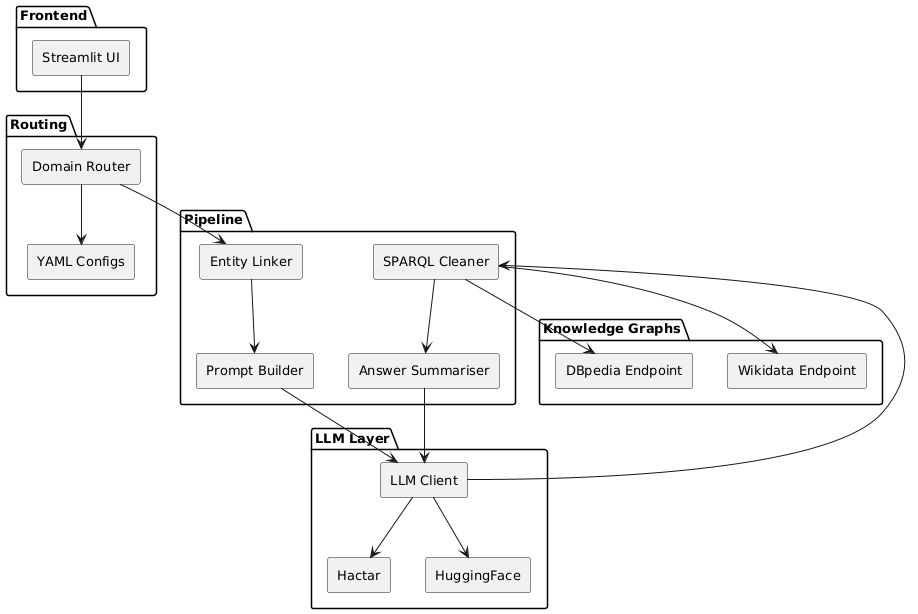
\includegraphics[width=0.95\linewidth]{arch_component.png}
    \caption{High-level component architecture of the NL$\leftrightarrow$SPARQL prototype.}
    \label{fig:architecture}
\end{figure}

The entry point is the Streamlit UI, where the user types their question and selects their domain and then passes on to the domain router. The router loads the corresponding domain configuration, a YAML file that includes the endpoint URL, prefix for the namespaces, ontology hints, and few-shot question--SPARQL pairs. This file is the extension point of the system: no code changes are required for adding a new domain, just a new YAML file.

After resolving the domain, the pipeline enters the entity and predicate resolution step. A lightweight LLM call first extracts the named entities and relational keywords from the user's question; those terms are then sent to the Wikidata search API, which returns verified QIDs and PIDs (Section~\ref{sec:entity-resolution}). This replaced an earlier design that relied on QIDs and PIDs hardcoded in the YAML domain configuration files. When both entity and predicate identifiers are resolved, the pipeline attempts a deterministic template query directly against the SPARQL endpoint \cite{w3c2013sparql}, skipping the main LLM call entirely. If that template query returns results, the pipeline returns immediately. Otherwise, the verified identifiers are passed to the prompt builder, which assembles the full prompt from system instructions, domain hints, few-shot examples, and the grounded entity block. The prompt is then sent to the LLM client, which routes it to Hactar or HuggingFace \cite{touvron2023llama} depending on availability and the user's model selection.

Finally, the model output is cleaned removing any markdown or prose and is then executed against the domain's SPARQL endpoint. In case the query executes successfully but yields no results, the pipeline retries once by calling the LLM again with the same prompt but at a higher temperature (0.7), allowing the model to produce a different query. A successful result is handed to the answer summariser, which generates a concise, natural language answer and the raw result table.

\begin{figure}[H]
    \centering
    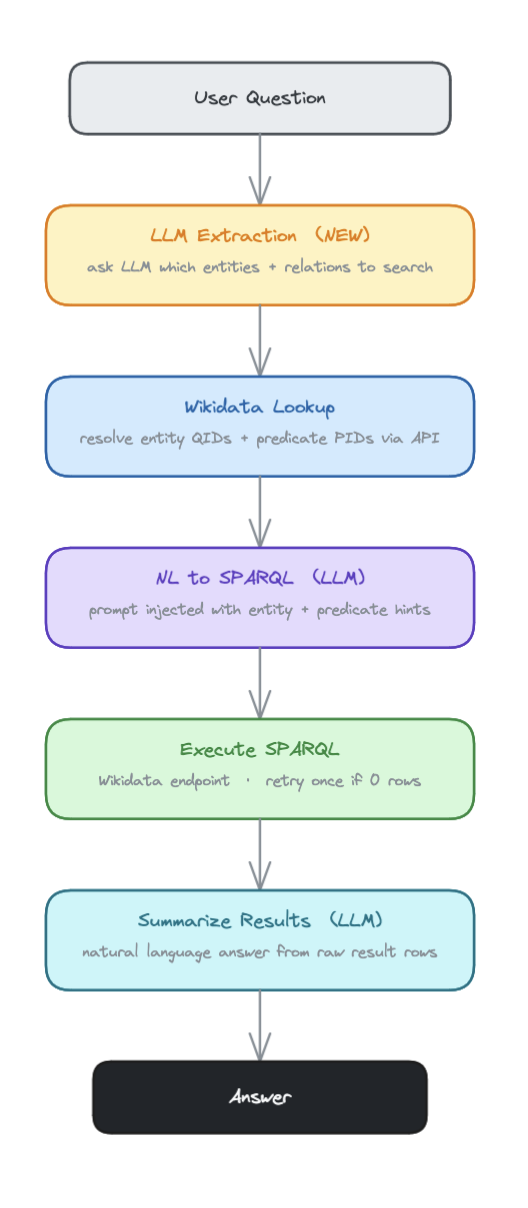
\includegraphics[width=0.55\linewidth]{arch_pipeline_v2.png}
    \caption{Updated pipeline activity diagram showing the new LLM extraction and Wikidata lookup steps, execution flow, and retry logic.}
    \label{fig:pipeline}
\end{figure}

\subsection{User Interface}
\label{sec:ui}

The interface is a single-page Streamlit application. The left side
of the screen is a fixed sidebar with the controls that apply to the
whole session, and the rest of the screen is a set of tabs, one for
each task. There are five tabs in total. This section covers the
three that do the actual translation and visualisation work. 

The sidebar is the same on every tab. At the top is the
\emph{Language Model} dropdown, which decides which LLM runs every
translation. Right below it is a status panel that lists the Hactar
models and the HuggingFace models, each with an \texttt{ONLINE} or
\texttt{OFFLINE} label and a refresh button. We added this panel
after getting tired of the same problem ourselves: Hactar goes down
fairly often (Section~\ref{sec:hactar}), and if the status is not
visible you only find out a model is dead after you have already
typed a question and waited for it to fail. Seeing which models are
up before running saves that wasted round-trip. Under \emph{Options}
there is one toggle, \emph{Summarize results in plain English},
which decides whether the user gets just the raw result table or
also a natural-language answer on top of it. We made this a choice
rather than always-on because the extra summary costs another LLM
call and not everyone wants it. Below that are a dark-mode toggle
and the two endpoint URLs, with the active endpoint shown in bold
and the inactive one greyed out so it is always clear where a query
is going.

\paragraph{Natural Language to SPARQL.}
This is the main tab and the one most users will spend their time
in. Above the input box there is a grid of example cards. Each card
has a domain tag (\textsc{Scientists \& Nobel Prizes},
\textsc{Movies}, \textsc{Music}, and so on), a difficulty tag
(\textsc{Simple}, \textsc{Lookup}, \textsc{Filter}, \textsc{Join},
\textsc{Aggregate}, \dots), the example question, and a
\emph{Use this} button that drops the question straight into the
input. The reason these cards are there is simple. An empty text box
tells the user nothing about what the system can do or how to ask
for it, and most people will not guess the phrasing that works best.
The cards show the range of each domain and a question shape that is
known to work. The difficulty tags are also a quiet warning: a
\textsc{Simple} list almost always works, while an
\textsc{Aggregate} or \textsc{Join} question is harder and fails
more often. Underneath the question box is the
domain dropdown. The figure below shows the tab with the sidebar on
the left and the example grid filled in.

% --- Figure: NL -> SPARQL tab (use the full-window screenshot that
%     also shows the sidebar, e.g. the "Scientists & Nobel Prizes"
%     view). Save it as figures/ui_nl2sparql.png and uncomment the
%     \includegraphics line.
\begin{figure}[H]
    \centering
    % \includegraphics[width=\linewidth]{ui_nl2sparql.png}
    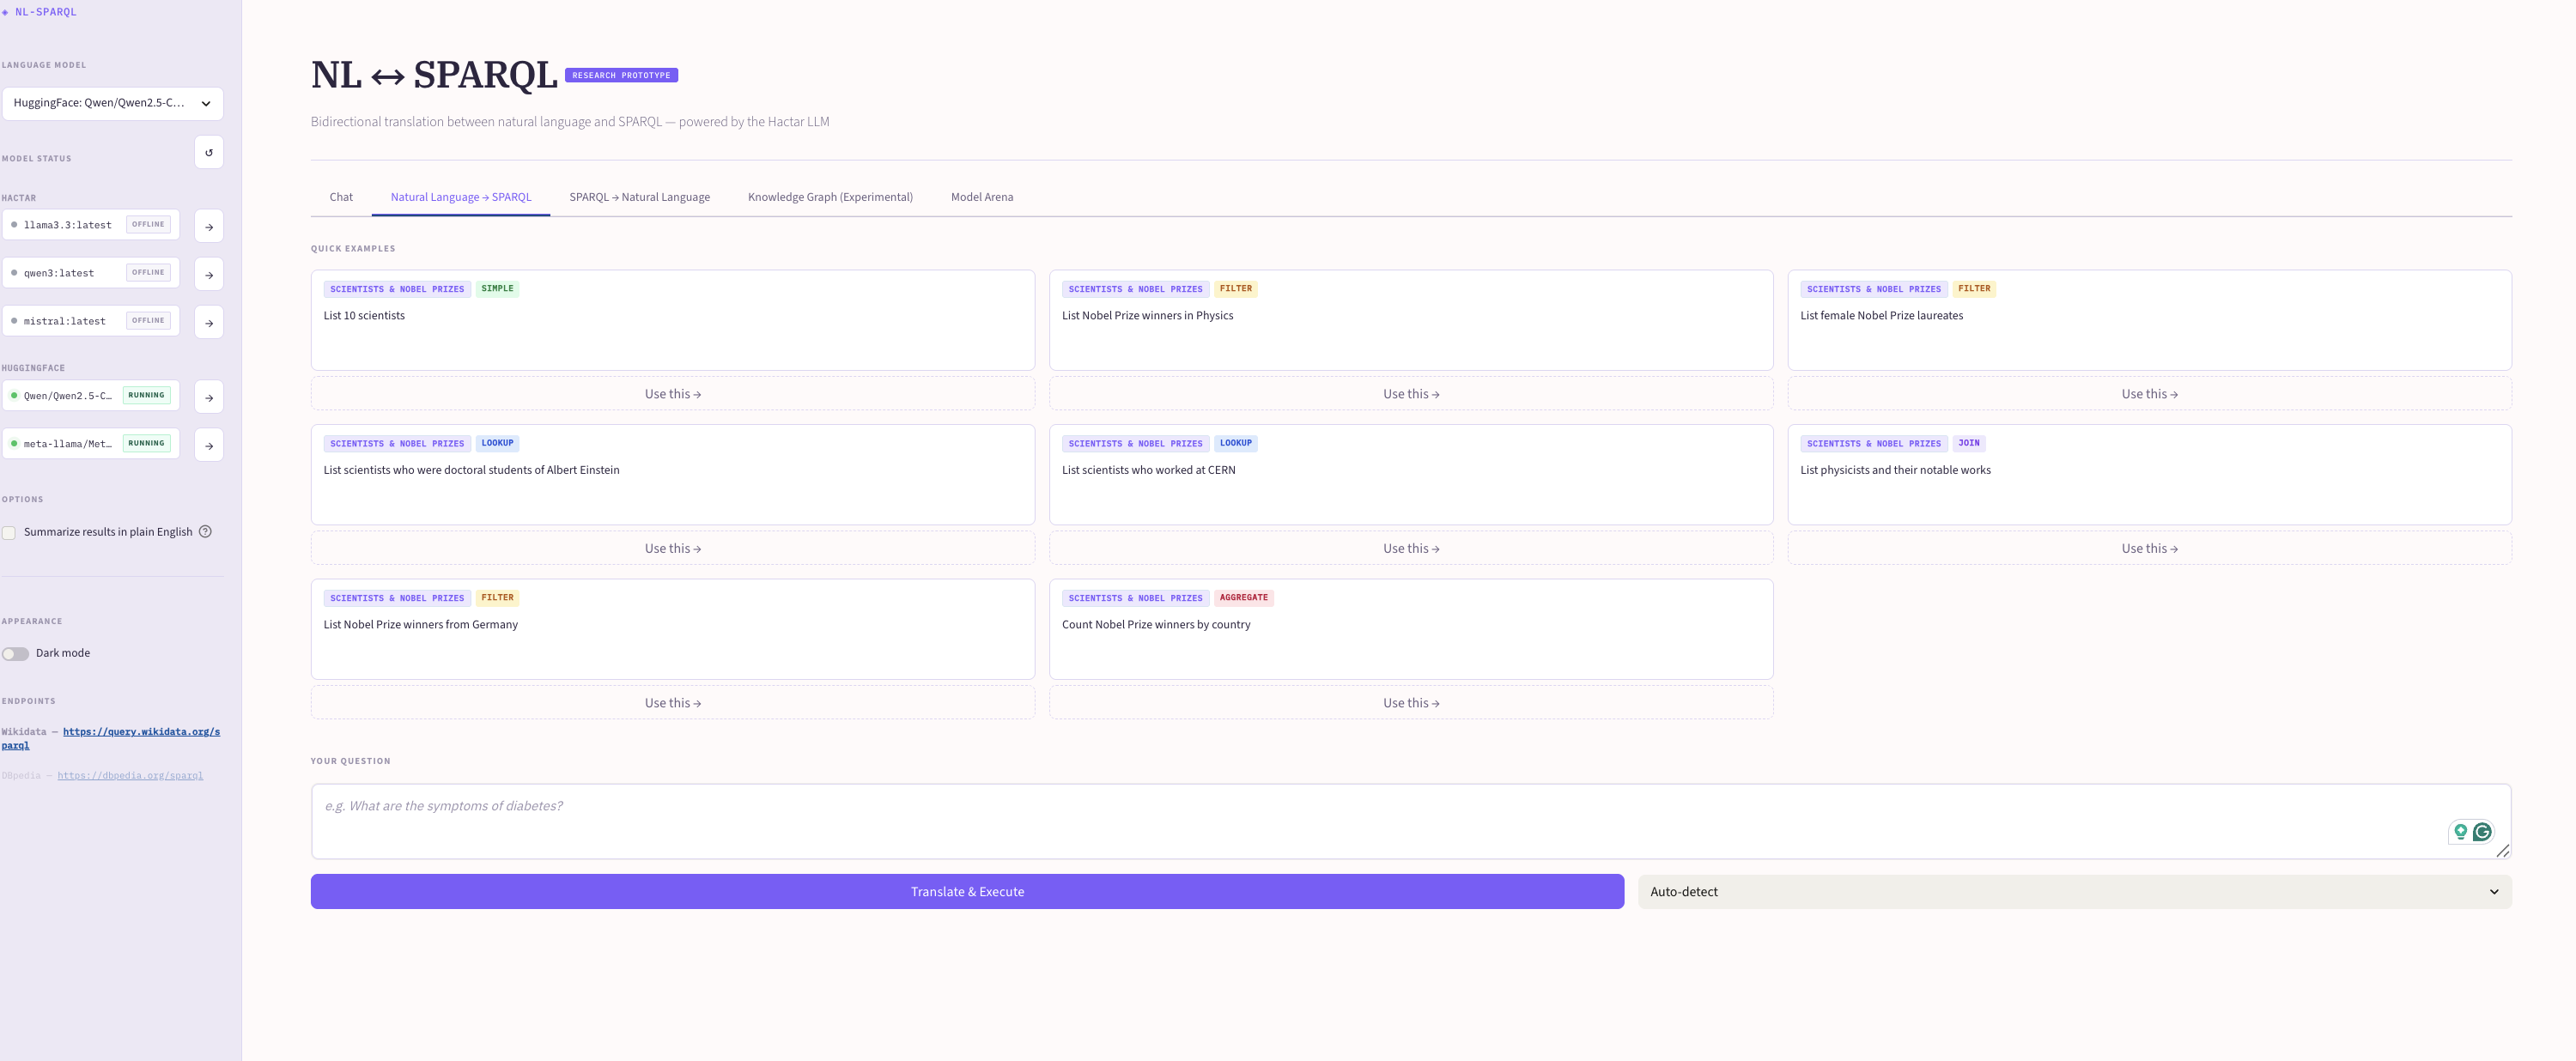
\includegraphics[width=0.92\linewidth]{figures/NL.png}
    \caption{The Natural Language $\rightarrow$ SPARQL tab, showing the global sidebar and the per-domain example cards.}
    \label{fig:ui-nl2sparql}
\end{figure}

The domain dropdown is worth a closer look because it carries a
design decision from Section~\ref{sec:routing}. The options are not
a flat list. They are split into a \emph{Wikidata} group and a
\emph{DBpedia} group with a separator line between them.

% --- Figure: domain dropdown open. Use one of the screenshots where
%     the grouped dropdown is expanded (Wikidata group / DBpedia
%     group with the separator). Save as figures/ui_domain_dropdown.png
\begin{figure}[H]
    \centering
    % \includegraphics[width=\linewidth]{ui_domain_dropdown.png}
    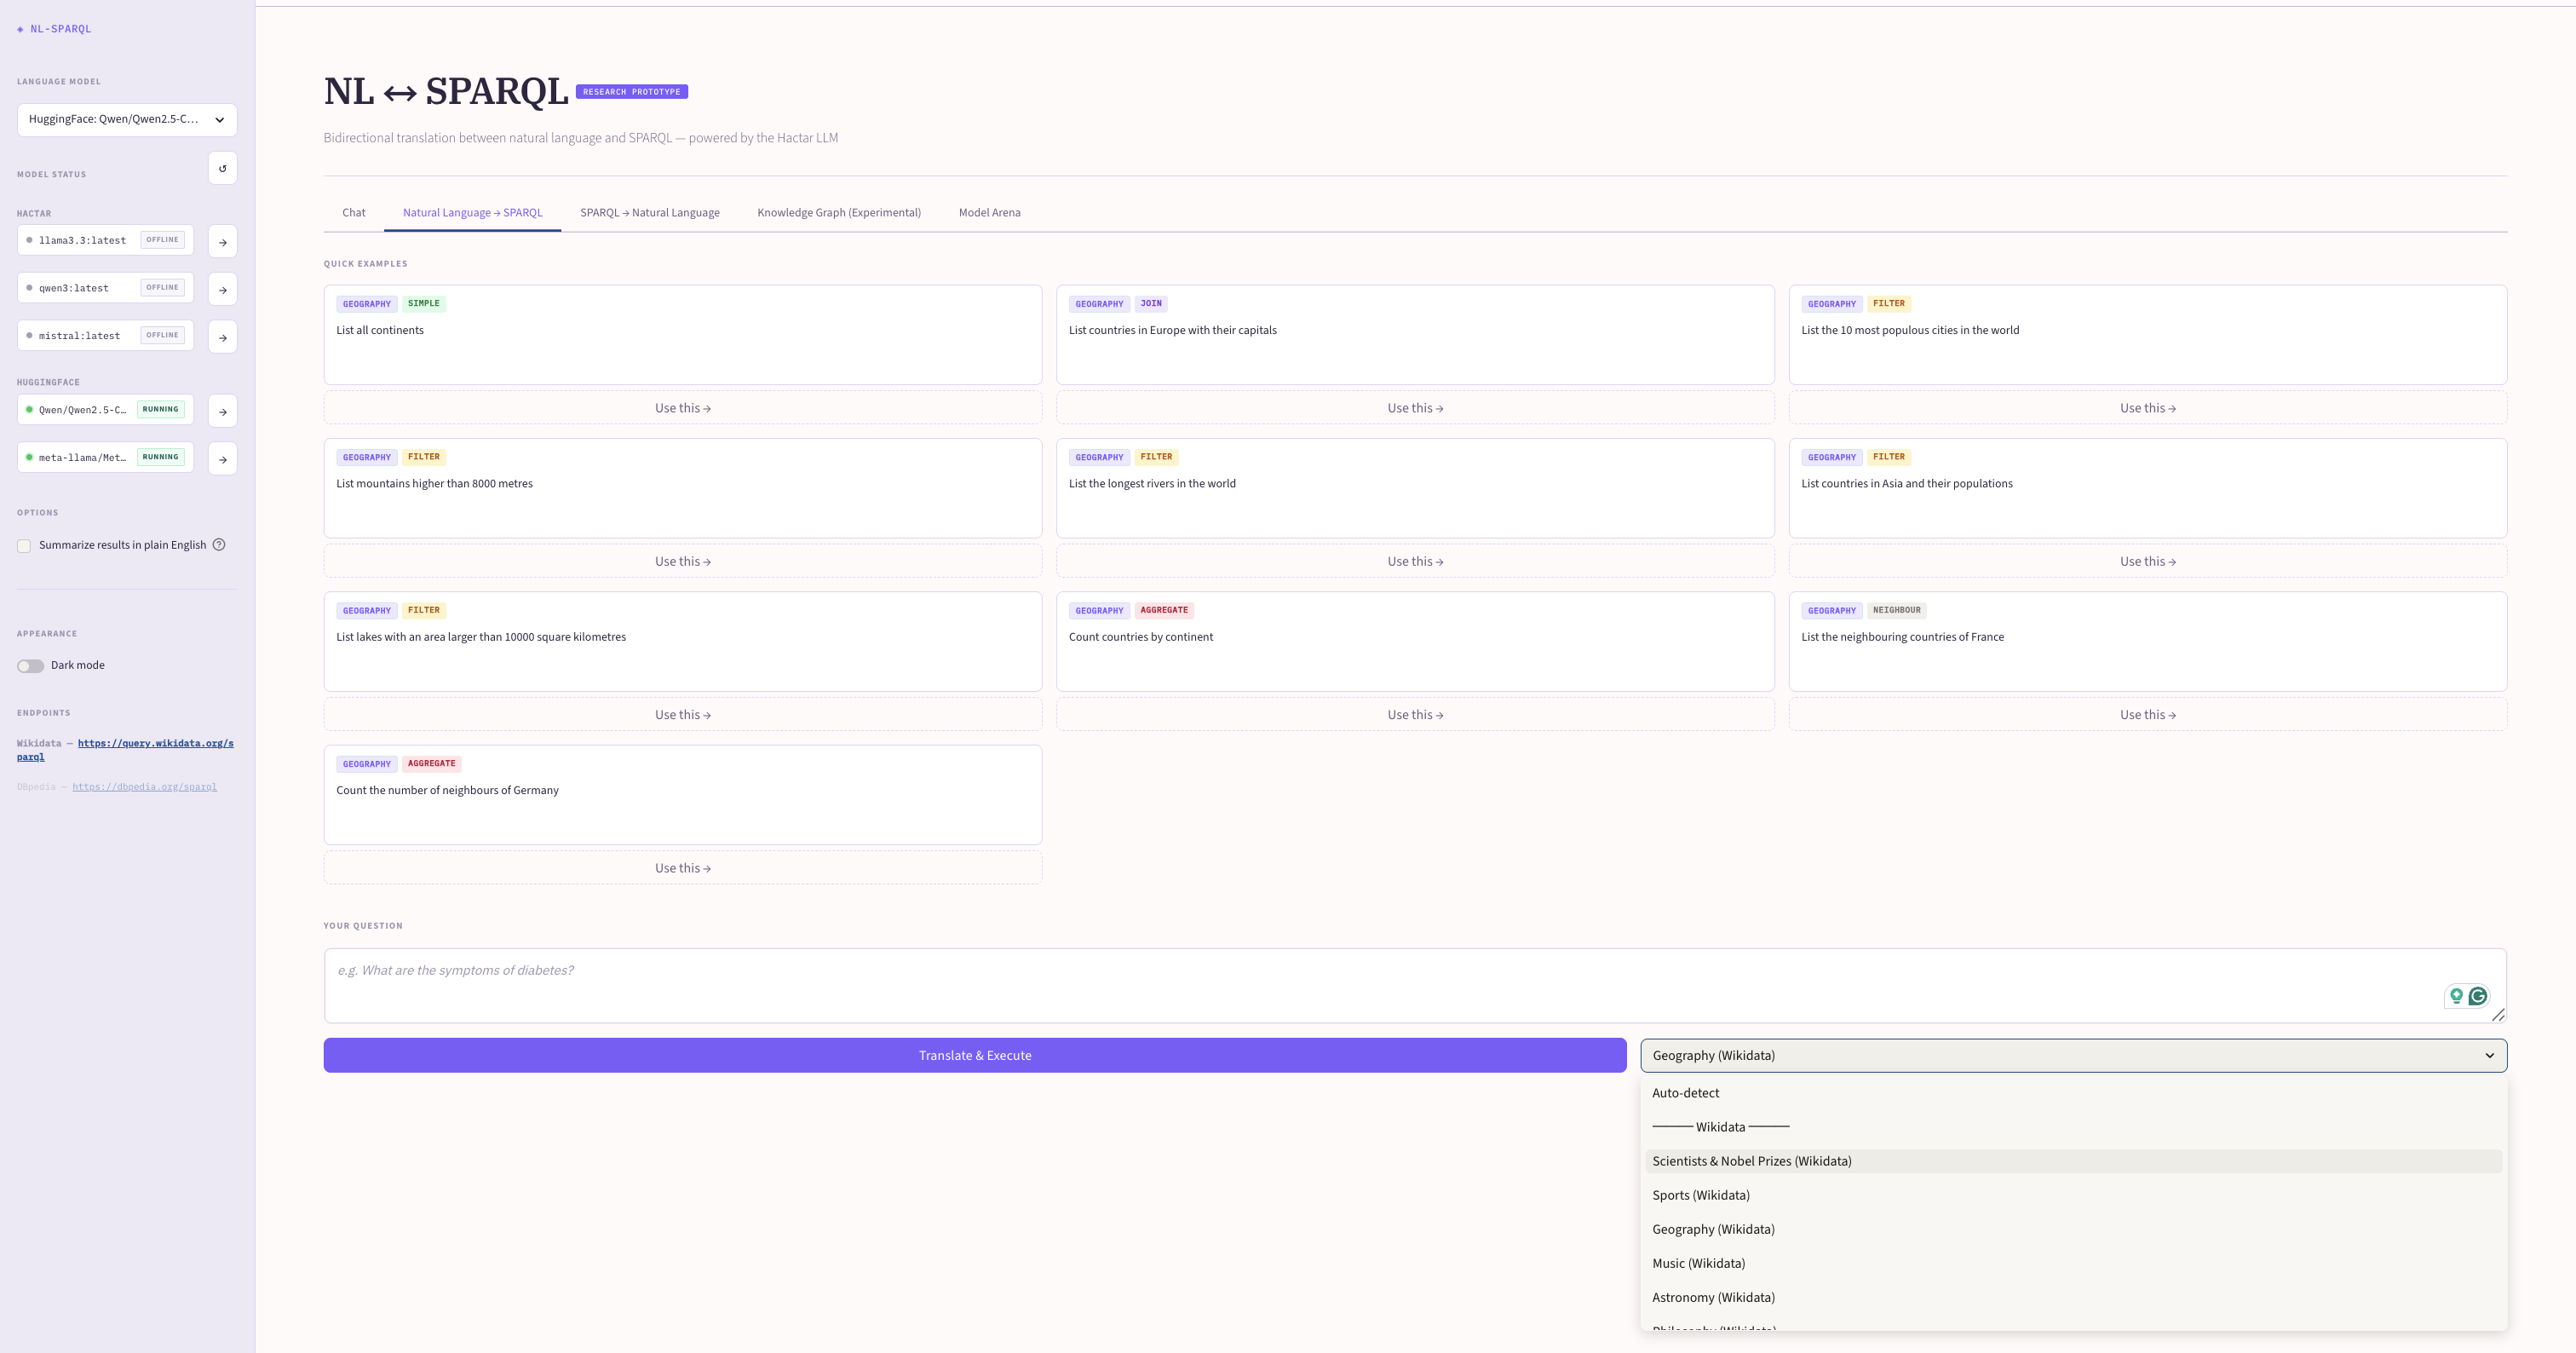
\includegraphics[width=0.92\linewidth]{figures/domain.png}
    \caption{The domain selector, grouped by knowledge base so the
    Wikidata/DBpedia split is visible at the point of selection.}
    \label{fig:ui-domain-dropdown}
\end{figure}




\begin{figure}[H]
    \centering
    % \includegraphics[width=\linewidth]{ui_domain_dropdown.png}
    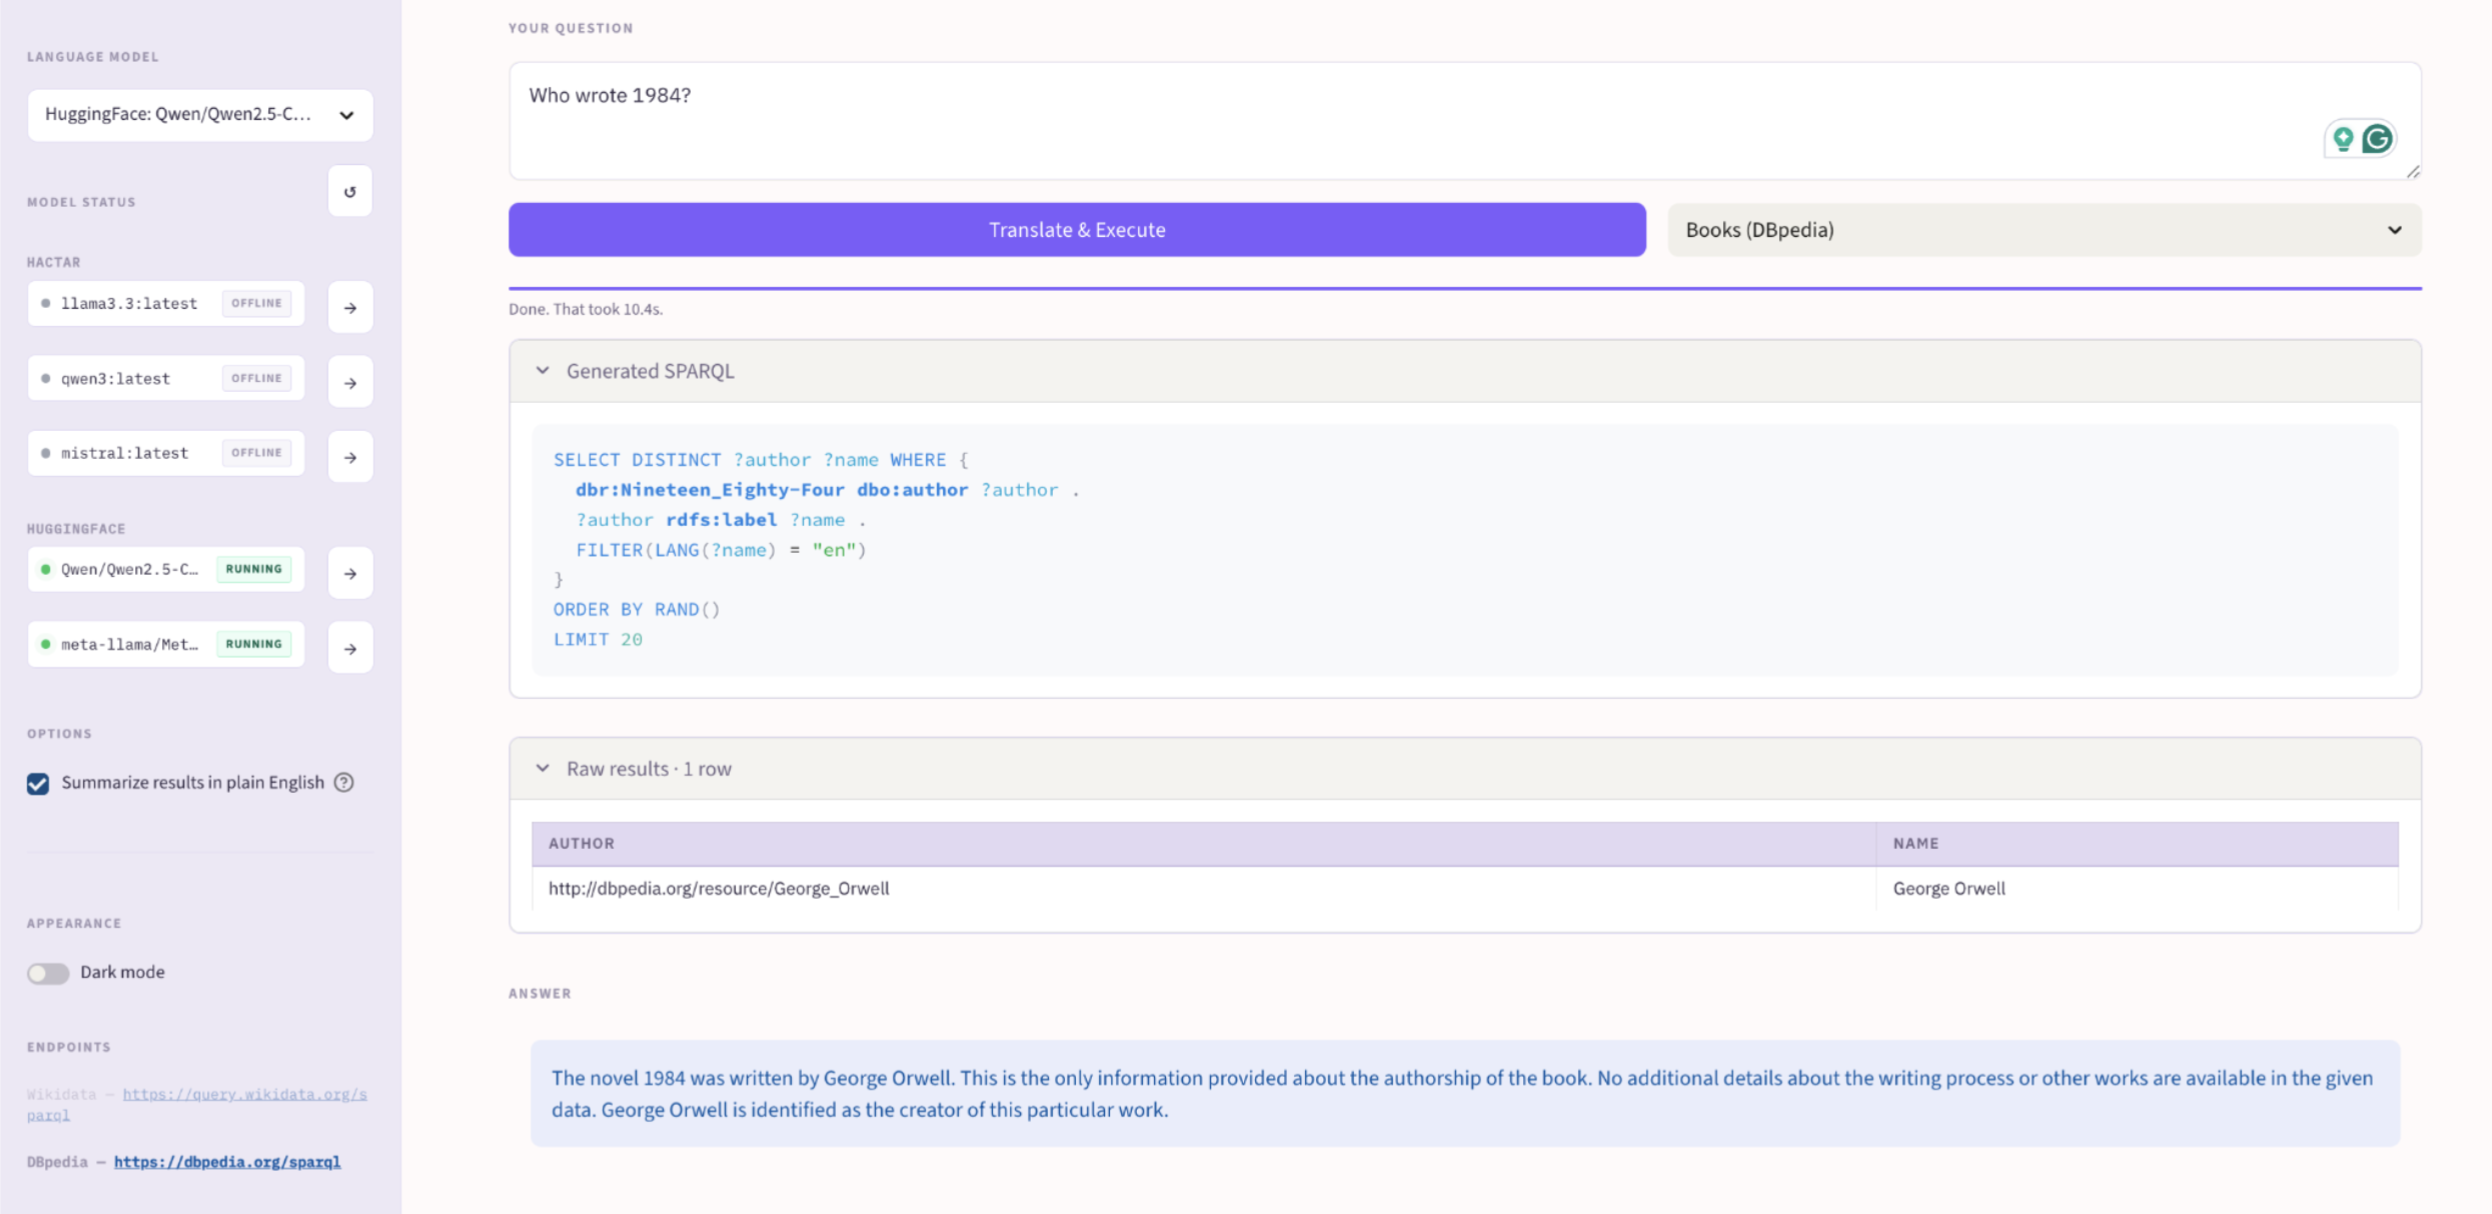
\includegraphics[width=0.92\linewidth]{figures/example.png}
    \caption{Example execution of the Natural Language $\rightarrow$ SPARQL pipeline in the Books domain using DBpedia. The system answers the question ``Who wrote 1984?'' by generating and executing a SPARQL query that retrieves George Orwell as the author.}
    \label{fig:ui-example}
\end{figure}



\paragraph{SPARQL to Natural Language.}
This tab is the first one turned around. It has the same kind of
example grid, except each card now has a \emph{Load query} button
that fills the box with a ready-made SPARQL query, one per domain.
The thinking is the same as on the other tab, just pointed the other
way: someone who wants to try the verbaliser probably does not have
a SPARQL query lying around to paste in, so we give them one for
every domain. Below the grid is the query box and an \emph{Explain
in English} button that runs the hybrid verbaliser from
Section~\ref{sec:sparql2nl}.

% --- Figure: SPARQL -> NL tab. Save as figures/ui_sparql2nl.png
\begin{figure}[H]
    \centering
    % \includegraphics[width=\linewidth]{ui_sparql2nl.png}
        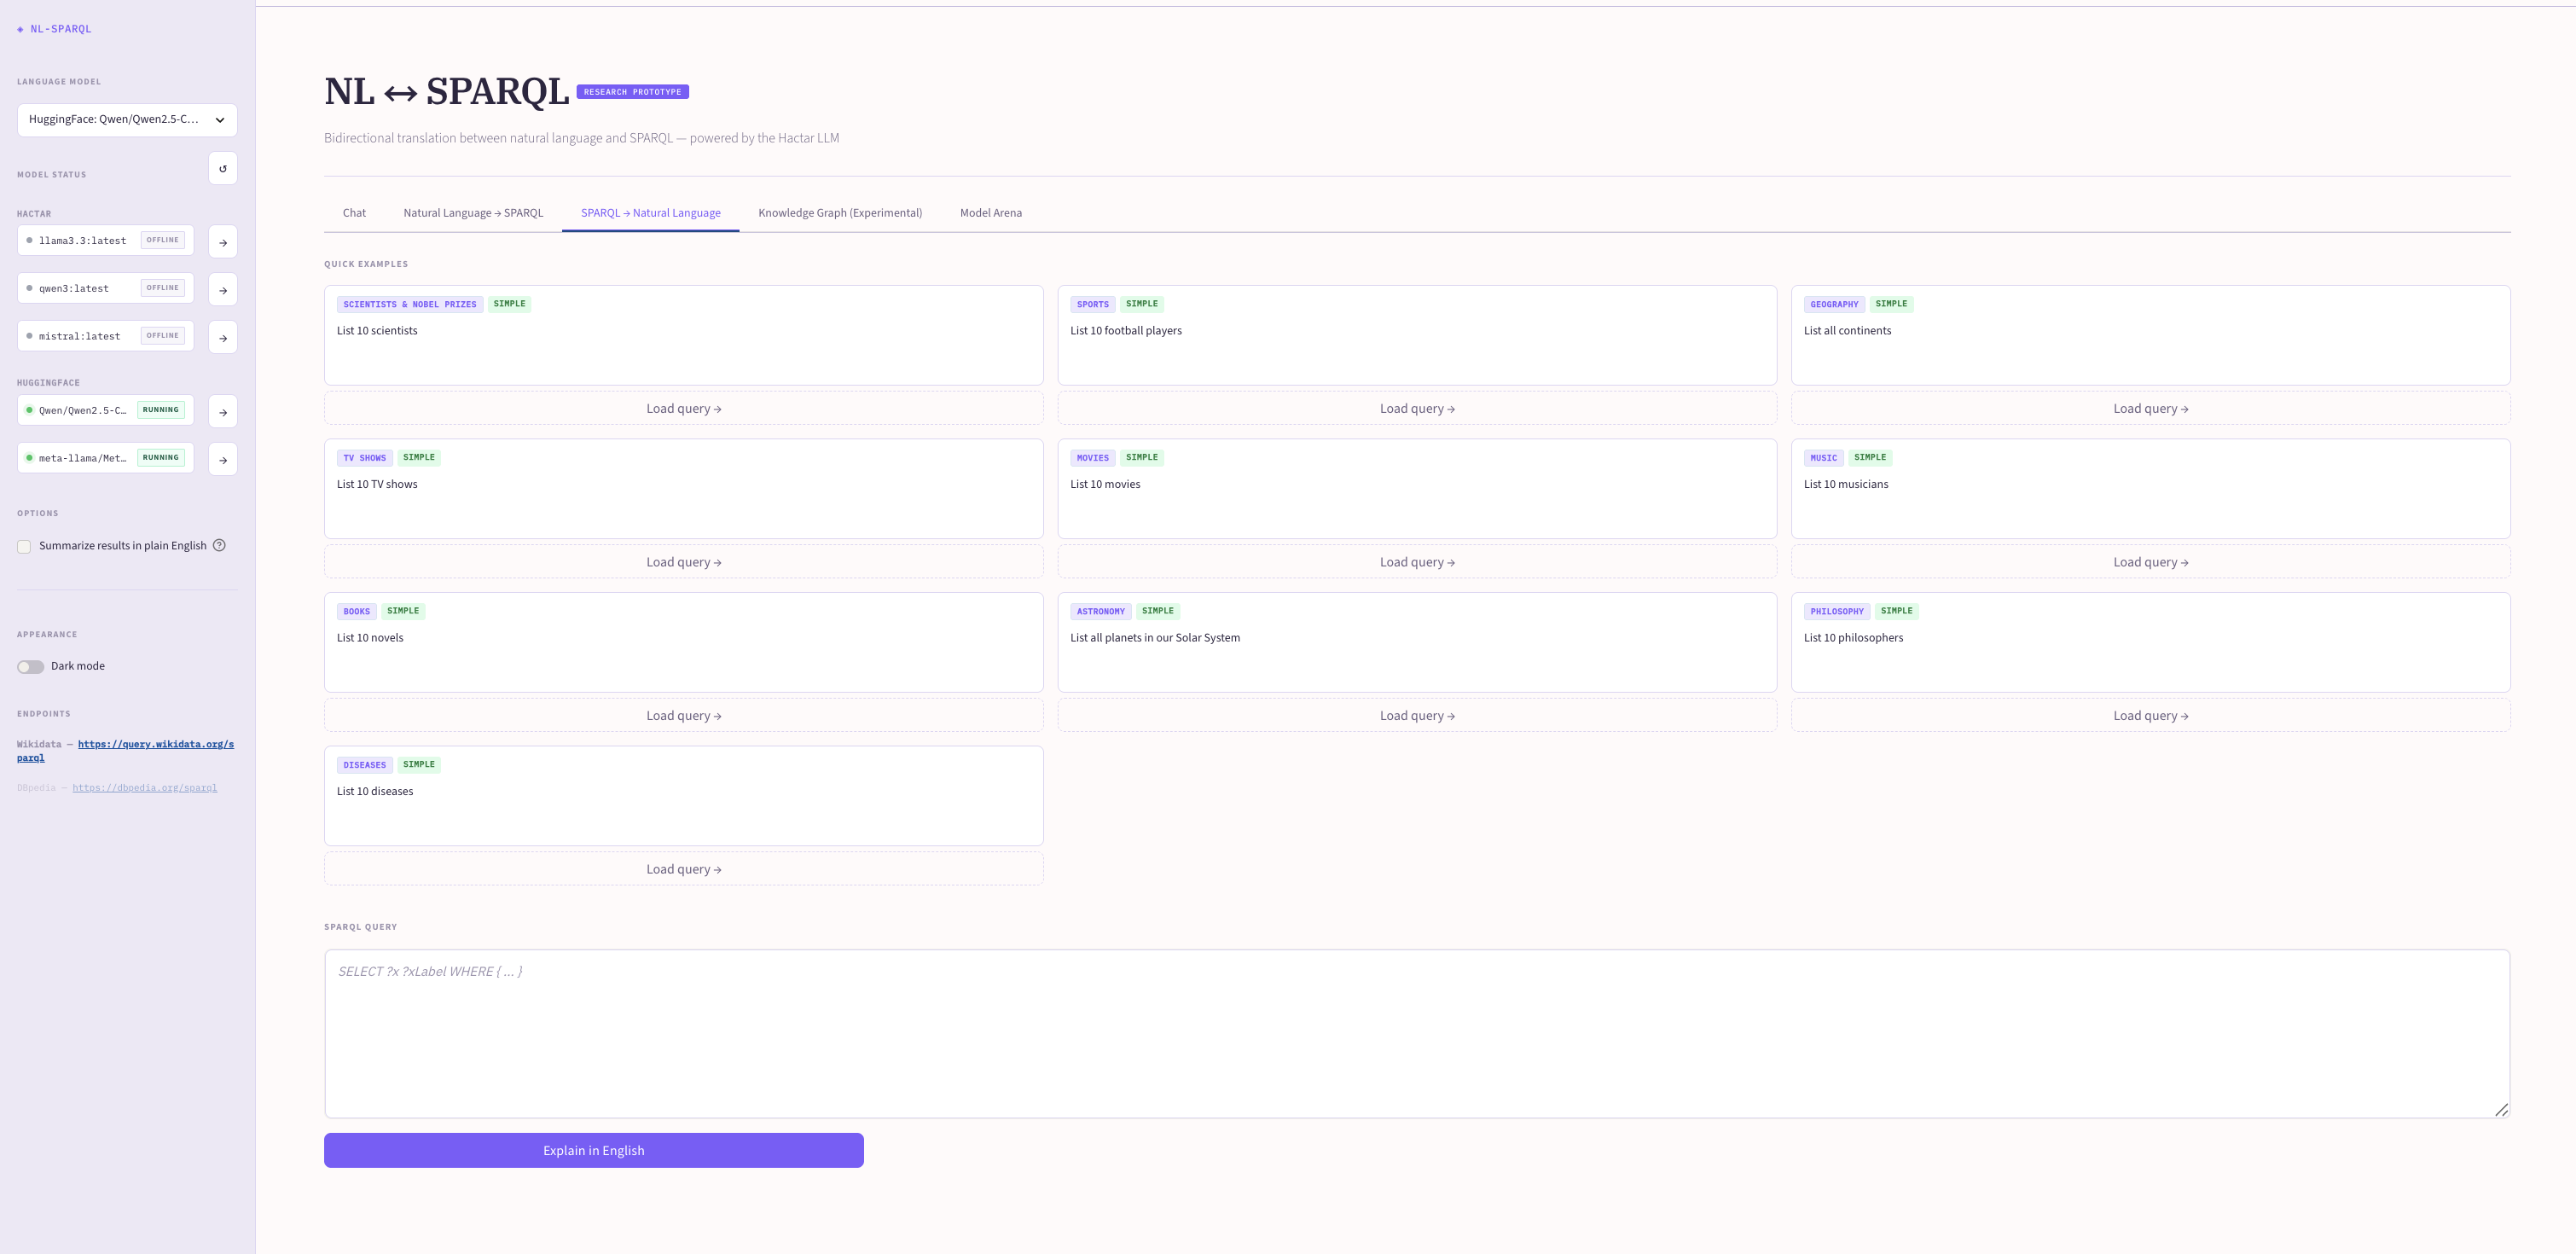
\includegraphics[width=0.92\linewidth]{figures/sparql.png}

    \caption{The SPARQL $\rightarrow$ Natural Language tab, with one
    ready-made query example per domain.}
    \label{fig:ui-sparql2nl}
\end{figure}

\paragraph{Knowledge Graph (Experimental).}
The last tab draws the results of a query as an interactive network.
Before the user runs anything there is a short note explaining the two modes, because the output shape
depends on the query and we would rather say that than have the user
be surprised by it. A query with two or more entity columns becomes
a relationship graph, and a flat single-column list becomes a star
graph around a central concept node (the reasoning behind the two
modes is in Section~\ref{sec:kgviz}). A row of example buttons fills
the query box with something that works, and after pressing
\emph{Visualize} the graph appears with a one-line summary above it
--- node count, edge count, average degree, and the most connected
node, for example \emph{Aristotle} in the philosopher-influence
example. That summary line is there so the user gets a quick sense
of the graph without having to read it node by node. A search box
helps find a node in a crowded graph, a \emph{Download Turtle}
button exports the same data for Prot\'eg\'e
(Section~\ref{sec:kgviz}), and the raw table and a path-finder are
tucked into collapsible panels below so they do not get in the way.

% --- Figure: Knowledge Graph tab. Save as figures/ui_kg.png
\begin{figure}[H]
    \centering
    % \includegraphics[width=\linewidth]{ui_kg.png}
        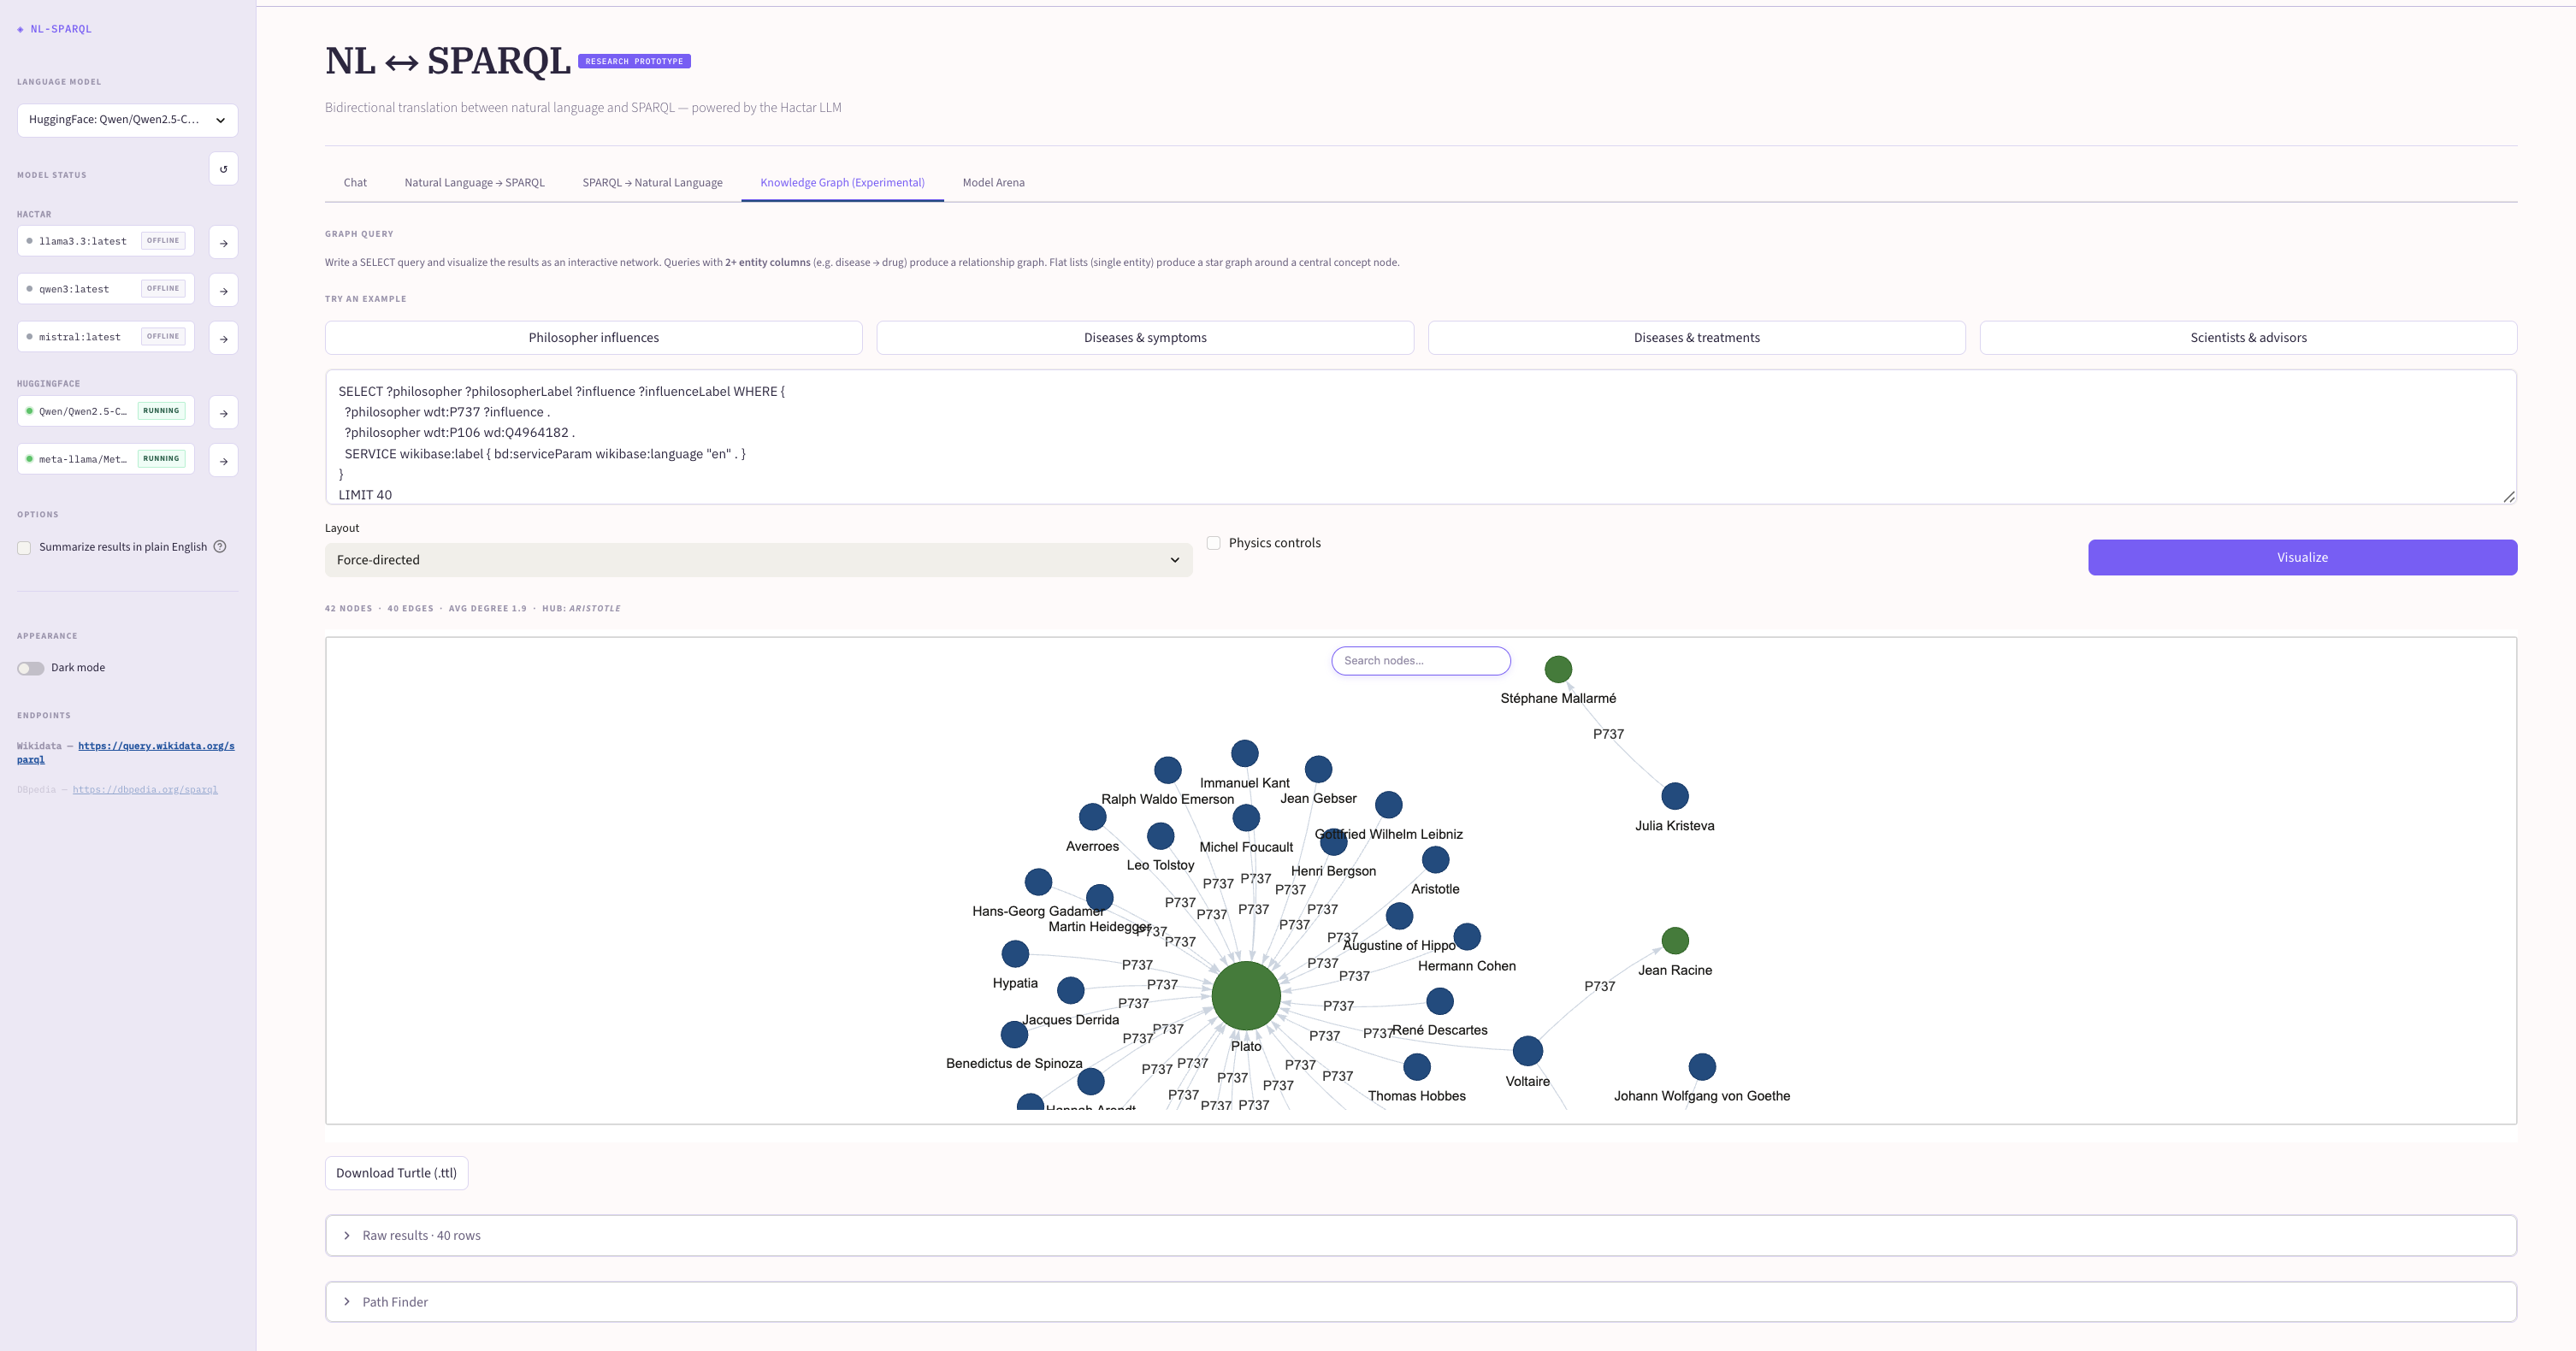
\includegraphics[width=0.92\linewidth]{figures/knowledgegraph.png}
    \caption{The Knowledge Graph tab rendering the
    philosopher-influence query as a star graph, with the summary
    line and Turtle export.}
    \label{fig:ui-kg}
\end{figure}










\subsection{Domain Configuration Files}
\label{sec:configs}

There is one YAML file in the configs/ directory for each domain in the system. The file contains all the elements that a pipeline should know to deal with that domain: the URL of the SPARQL endpoint \cite{w3c2013sparql}, the set of namespace prefixes to be used in the automatically generated queries, a block of ontology hints that provides a description of the most relevant classes and properties, a list of few-shot question--SPARQL pairs \cite{brown2020gpt3} that are presented as an example in the prompt, and a list of example questions that are displayed in the UI. To add a new domain, it is enough to drop in a new YAML file; no code changes are required. The split between the domain and pipeline code is deliberate: the prompt engineering all resides in the YAML file, allowing a domain expert to tweak or expand a domain without touching any Python.

\begin{lstlisting}[style=plainStyle, caption={Skeleton of a domain
YAML configuration file.}, label={lst:domain-yaml}]
domain_name: "Books (DBpedia)"
description: "Literature domain using DBpedia: ..."
endpoint: "https://dbpedia.org/sparql"

prefixes: |
  PREFIX dbo: <http://dbpedia.org/ontology/>
  PREFIX dbr: <http://dbpedia.org/resource/>
  PREFIX dbp: <http://dbpedia.org/property/>

ontology_hints: |
  Key DBpedia classes and properties:
  - dbo:Book    = "a book"
  - dbo:Writer  = "a writer or author"
  - dbo:author  = "author of the book"
  - dbo:genre   = "literary genre"

few_shot_examples:
  - question: "Who wrote 1984?"
    tag: "Lookup"
    sparql: |
      SELECT DISTINCT ?author ?name WHERE { ... }

example_questions:
  - question: "List 10 novels"
    tag: "Simple"
\end{lstlisting}

Currently, the system has 10 domains in the two knowledge graphs. Three target DBpedia:

\begin{itemize}
    \item \textbf{Books}: which focuses on authors, genres and publishers with the \texttt{dbo:Writer} and \texttt{dbo:Book} classes
    \item \textbf{Movies}: which focuses on directors, actors, release dates and box office data
    \item \textbf{TV Shows}: which focuses on series, seasons, episodes, cast and broadcast networks
\end{itemize}

The other seven are:

\begin{itemize}
    \item \textbf{Diseases}: condition, symptom, treatment and ICD-10 codes from the biomedical domain
    \item \textbf{Music}: artists, bands, albums, songs, and genres
    \item \textbf{Philosophy}: philosophers, philosophy schools, and influences
    \item \textbf{Sports}: athletes, teams, competitions
    \item \textbf{Scientists \& Nobel Prizes}: researchers, laureates, institutions
    \item \textbf{Astronomy}: planets, stars, moons, galaxies, and other celestial bodies
    \item \textbf{Geography}: countries, cities, continents
\end{itemize}

The DBpedia domains \cite{auer2007dbpedia} have prefix \texttt{dbo:}, \texttt{dbr:}, and \texttt{dbp:} and depend on the readable names of properties, whereas the Wikidata domains \cite{vrandecic2014wikidata} use entity-looked-up Q-IDs, with P-IDs.

% ============================================================
\subsection{Model Arena}
\label{sec:arena}
% ============================================================

The Model Arena tab allows the user to run the same natural-language question through several language models simultaneously and compare their outputs side by side. The motivation is straightforward: no single model is reliably best for all question types, and the only honest way to assess this is to run them in parallel on the same input and inspect the results together.

\paragraph{Model selection and parallel execution.}
At the top of the tab the user selects which models to include using a multiselect widget. This step is practical rather than aesthetic: some servers are intermittently unavailable, and excluding a known-down model prevents the whole comparison from stalling. Once the selection is confirmed and the question is submitted, each model runs in a separate thread using Python's \texttt{ThreadPoolExecutor}, so the slowest model does not block the others. Each thread follows the same pipeline as the main translation tab: the question is translated to SPARQL, the query is cleaned and executed, and if the endpoint returns an error or zero rows the system automatically retries using a label-based fallback prompt. The per-model wall-clock time is recorded for comparison.

\paragraph{Per-model result panel.}
After execution, each model is shown in its own expandable panel (Figure~\ref{fig:arena1}). The panel displays the generated SPARQL query, a one-sentence explanation of what the query retrieves (produced by a second LLM call), the result rows returned by the endpoint, and a natural-language answer synthesised from those rows. A \emph{Retried} badge appears when the fallback prompt was needed.

\begin{figure}[H]
    \centering
    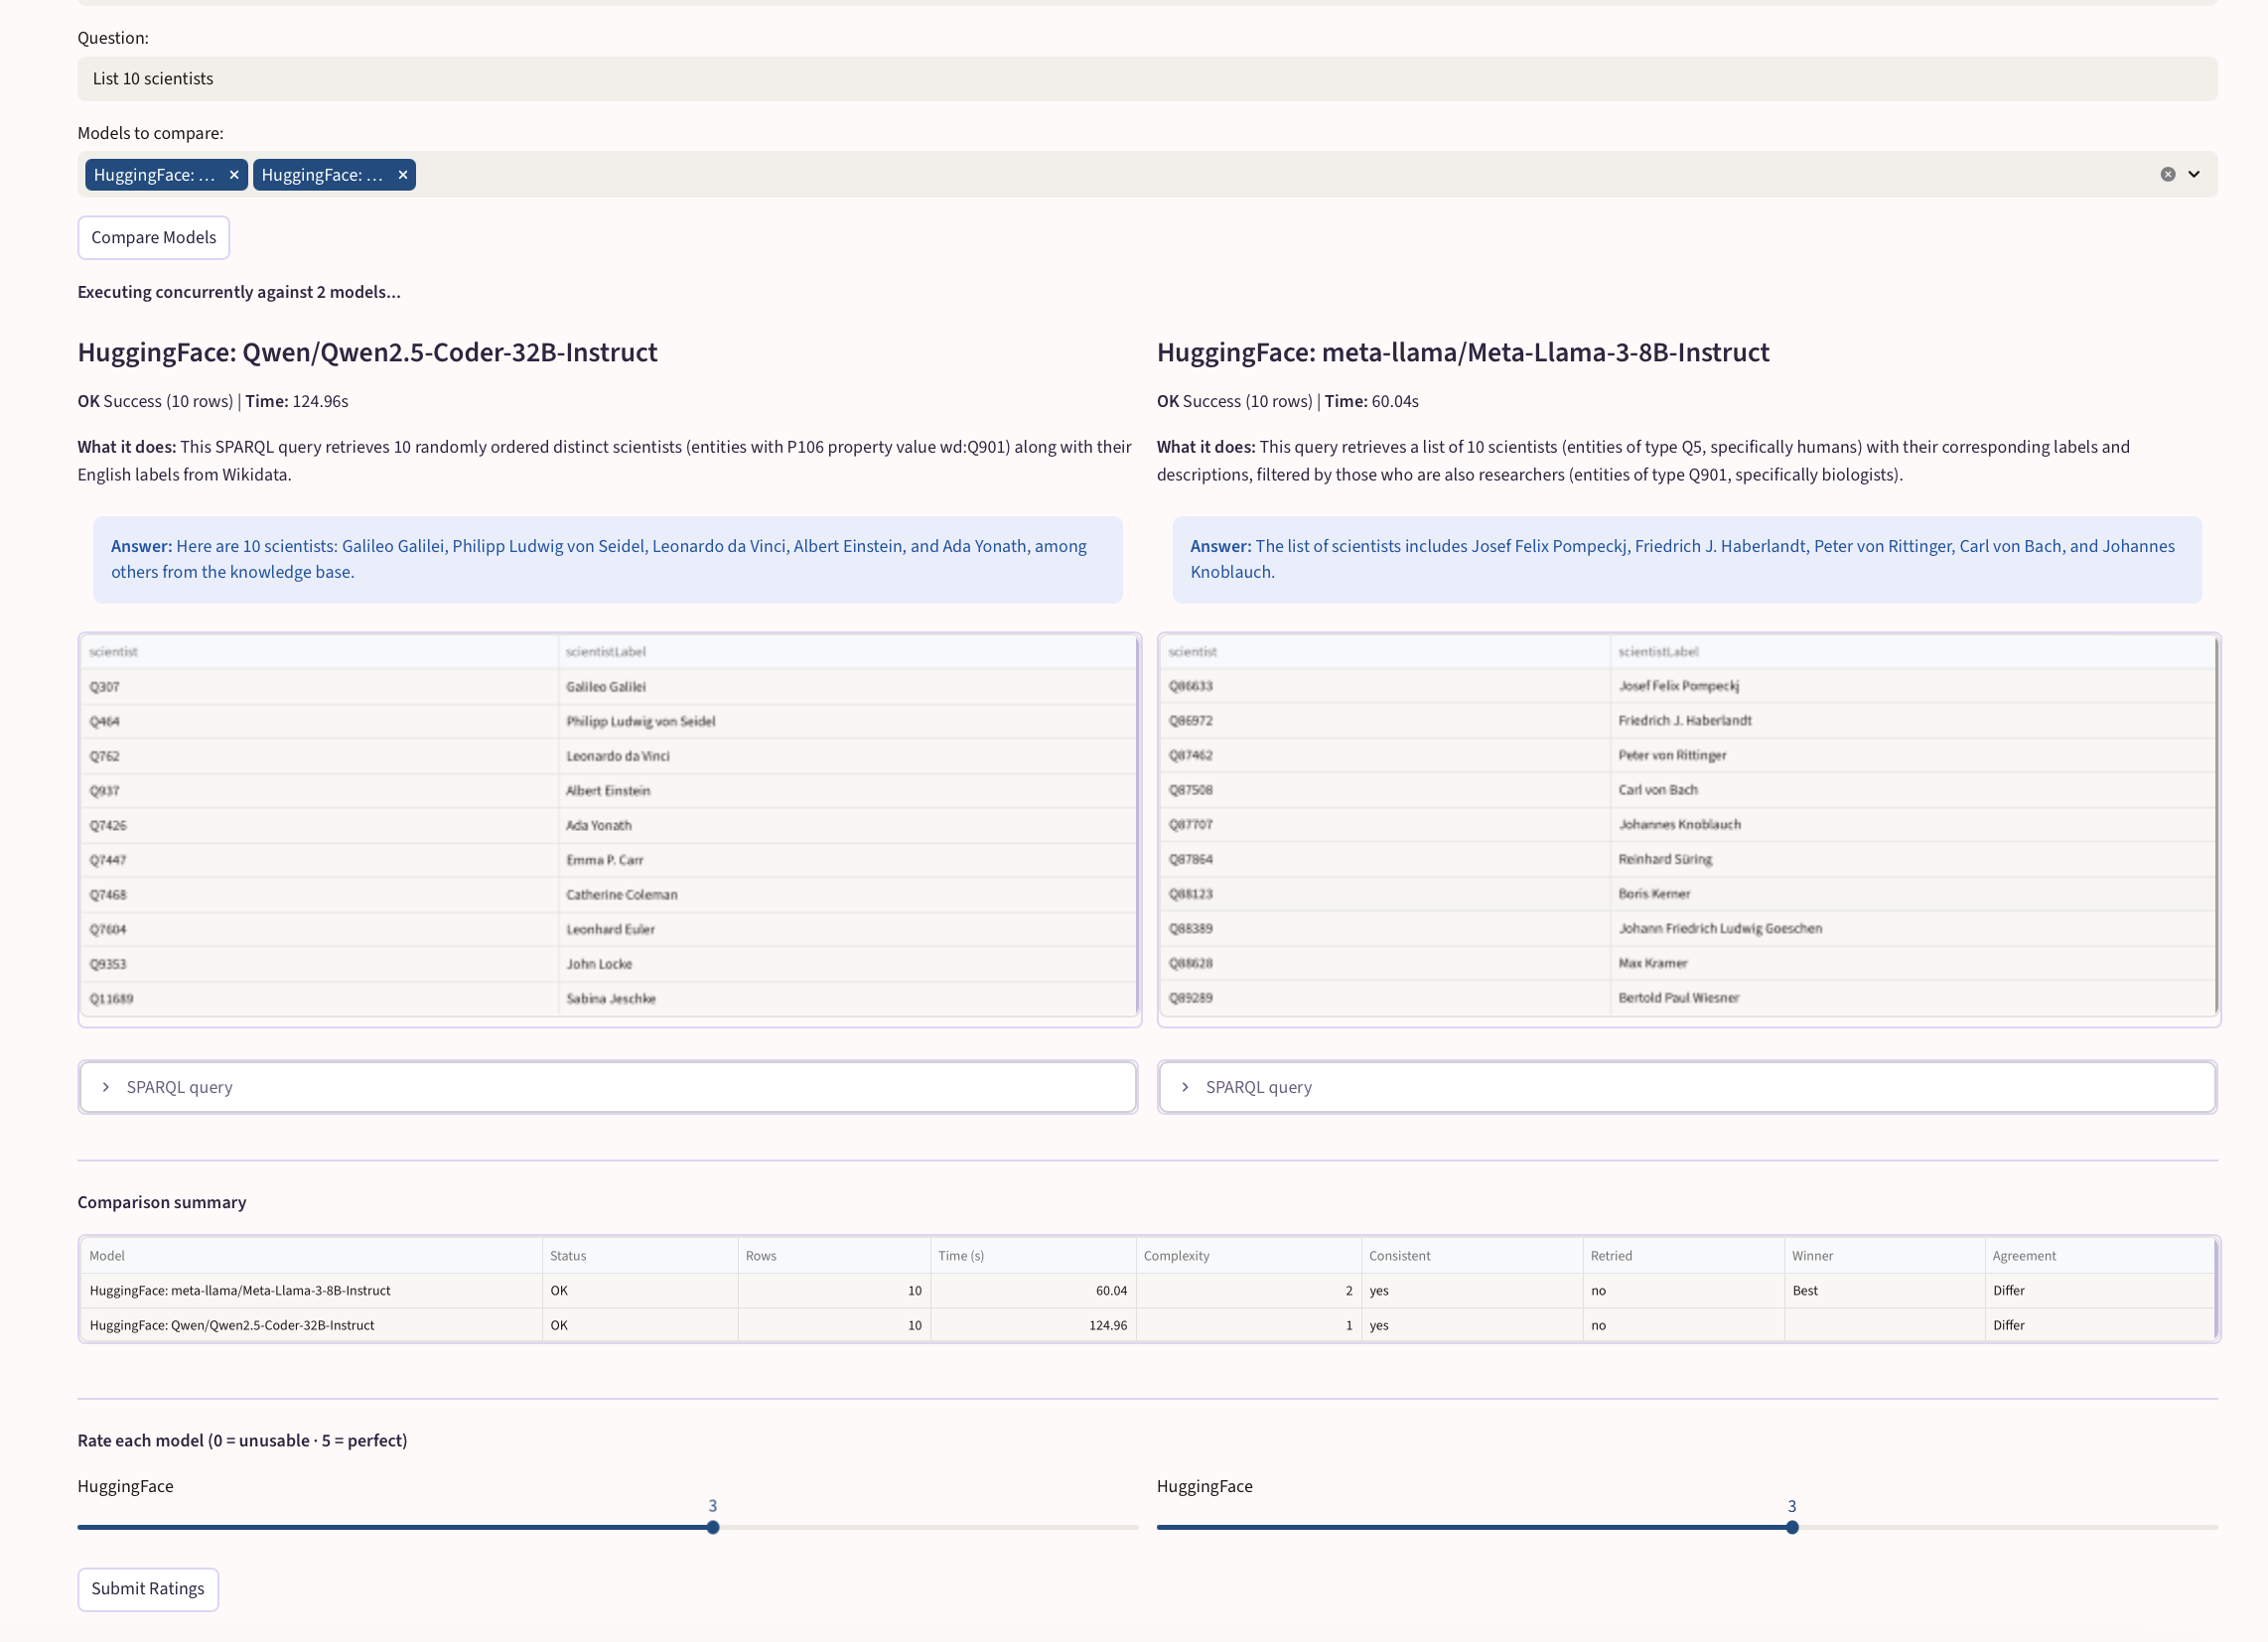
\includegraphics[width=0.95\linewidth]{figures/arena1.png}
    \caption{The Model Arena tab after running a question through two models. Each model panel shows its SPARQL query, a one-sentence explanation, the result rows, and a natural-language answer. The rating sliders appear below.}
    \label{fig:arena1}
\end{figure}

\paragraph{Comparison summary table.}
Below the individual panels, a summary table brings all models together in one view. It reports, for each model: execution status, number of rows returned, wall-clock time, SPARQL complexity (number of triple patterns), whether the answer was consistent across two independent runs of the same question, whether a retry was needed, a \emph{Best} badge for the fastest successful model, and whether all models agreed on the same first answer.

\paragraph{User ratings and feedback.}
After reviewing the results, the user can rate each model on a 0--5 scale (Figure~\ref{fig:arena2}). On submitting the ratings, a second step collects structured feedback: for models rated 3 or higher, a set of positive reasons is shown (e.g.\ \emph{Correct answer}, \emph{Clear explanation}, \emph{Good SPARQL structure}); for models rated below 3, a set of negative reasons is shown (e.g.\ \emph{Wrong or empty answer}, \emph{Bad SPARQL}, \emph{Too slow}). The user can also type a free-text comment for each model (Figure~\ref{fig:arena3}). All ratings and feedback are appended to a local JSON file so that the leaderboard, shown at the bottom of the tab, persists across sessions.

\begin{figure}[H]
    \centering
    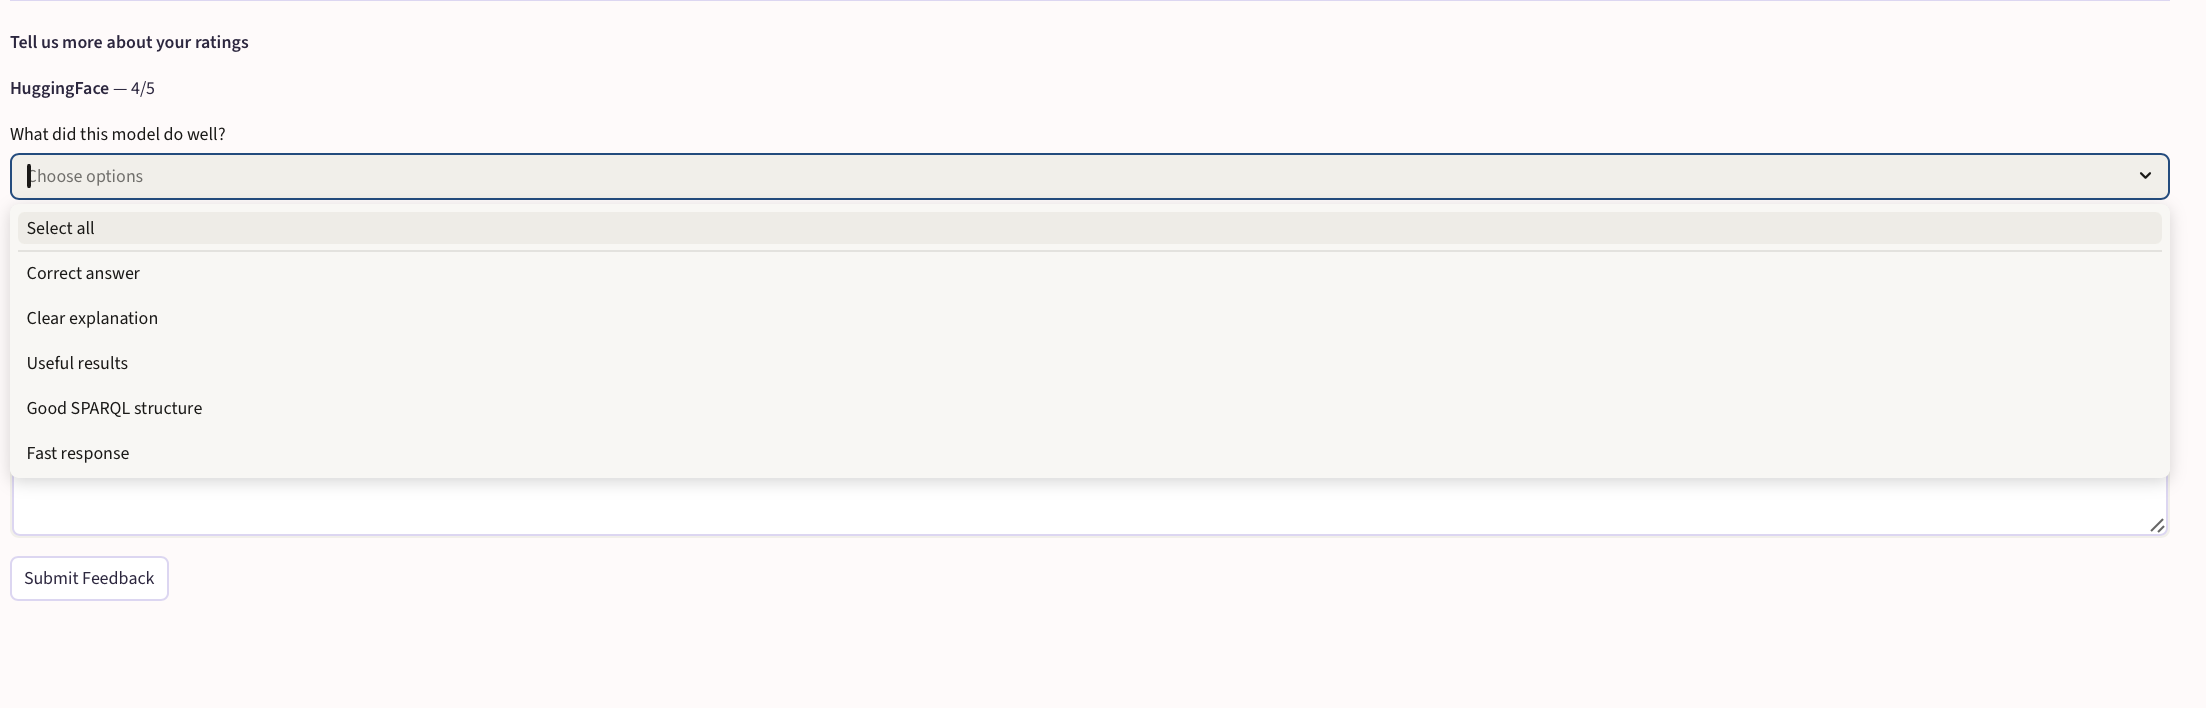
\includegraphics[width=0.95\linewidth]{figures/arena2.png}
    \caption{The feedback step for a model rated 4 out of 5. The user selects reasons from a predefined list and can add a free-text comment.}
    \label{fig:arena2}
\end{figure}

\begin{figure}[H]
    \centering
    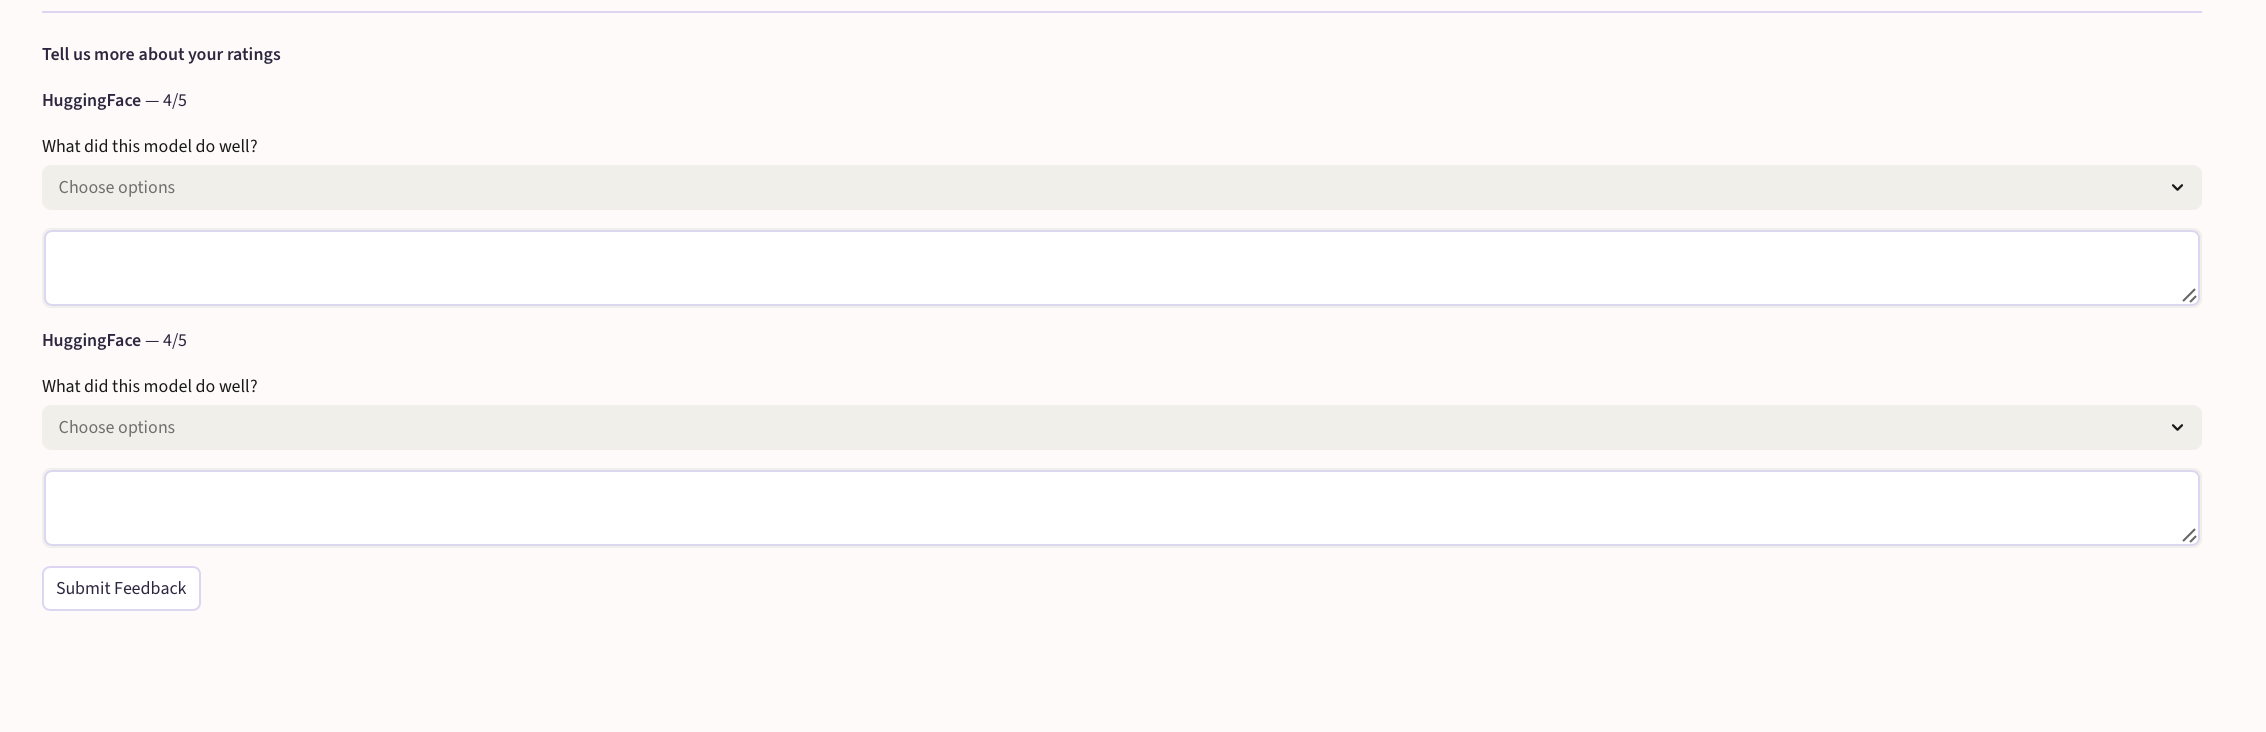
\includegraphics[width=0.95\linewidth]{figures/arena3.png}
    \caption{The feedback form showing both models side by side, each with its rating, reason checkboxes, and comment field.}
    \label{fig:arena3}
\end{figure}

% ============================================================
\section{Methodology}
\label{sec:methodology}
% Suggested length: ~1500-1800 words. This is the heart of the
% paper. Each subsection corresponds to one engineering choice
% with a justification (cite a paper or course material when you
% can).
% ============================================================

This section describes the methodology used to build the bidirectional Natural Language to SPARQL system, covering the three main components: domain routing (which lets the user choose the domain from a dropdown grouped by knowledge base), Natural Language to SPARQL translation, and SPARQL to Natural Language translation.

\subsection{Domain Routing}
\label{sec:routing}

Domain routing is the first step of the pipeline because the selected domain determines how the rest of the system behaves. Before a SPARQL query can be generated, the system needs to know which knowledge base, endpoint, prefixes, ontology hints, and examples should be used. For this reason, domain routing acts as a bridge between the user's natural language question and the domain-specific configuration required for query generation.

The system uses manual domain selection which lets the user to choose the domain that the question belongs to from a dropdown that is grouped under Wikidata and DBpedia section headers, as well as an automatic detection option.

Having a manual domain selection is important because the selected domain controls several technical components of the pipeline. First, it determines the SPARQL endpoint to which the generated query will be sent. For example, the diseases domain is connected to Wikidata, while the movies domain is connected to DBpedia. Therefore, selecting a domain does not only categorize the question conceptually, but also routes the query to the appropriate knowledge base.

Second, the domain selection affects the prefixes and vocabulary used in the generated SPARQL query. Wikidata and DBpedia use different schemas and different property structures. For instance, DBpedia commonly uses prefixes such as \texttt{dbo:}, while Wikidata relies on structures such as \texttt{wdt:} and \texttt{wd:}. If the wrong domain is selected, the model may generate a query with prefixes or properties that are not compatible with the selected endpoint.

Third, domain selection also influences the few-shot examples given to the LLM. These manually added extra example questions for each domain in order to help users understand what kinds of questions they can ask within the system. These questions are not generated automatically; instead, they are manually defined inside each domain configuration YAML file under the \texttt{example\_questions} section.

For example, in the \texttt{wikidata\_diseases.yaml} configuration file, I added questions such as:

\begin{itemize}
    \item ``List 10 diseases''
    \item ``What are the symptoms of diabetes?''
    \item ``Which drugs are used to treat malaria?''
    \item ``Find diseases that affect the lungs''
    \item ``Which diseases are caused by bacteria?''
\end{itemize}

For the Auto-detect option, the idea is that the LLM would read the user's question, decide which domain it belonged to, and continue with that domain's configuration.

The main motivation behind this feature was to reduce the risk of user error during domain selection. In the earlier version, the user had to manually choose the correct domain before asking a question. However, if the user selected the wrong domain, the system could send the query to an unsuitable endpoint or use an incompatible configuration.

With the new design, manual domain selection still remains available, but the user can also choose the Auto option. When Auto-detect is selected, the system first analyzes the user’s natural language question and asks the LLM to predict the most appropriate domain. After identifying the domain, the system automatically continues with the corresponding domain configuration, including the correct endpoint, prefixes, ontology hints, and few-shot examples.

For example, if the user asks:

\begin{quote}
Who directed Memento?
\end{quote}

the system should recognize that this is a movie-related question and select the Movies (DBpedia) domain. After that, it uses the movie domain configuration to generate and execute the SPARQL query. The interface also informs the user about this decision by displaying a message such as:

\begin{quote}
Auto-detected domain: Movies (DBpedia)
\end{quote}

This makes the system more transparent because the user can see which domain was selected automatically.

To test this feature, I used example questions from different categories, such as:

\begin{itemize}
    \item ``Who directed Memento?''
    \item ``Top 10 planets''
    \item ``Who influenced Kant?''
\end{itemize}

These examples were chosen because they clearly belong to different domains: movies, astronomy, and philosophy. This allowed me to check whether the automatic detection mechanism could distinguish between different types of user questions and route them to the correct domain configuration.

If the user selects a domain manually instead of using Auto-detect, the previous behavior remains unchanged. The selected domain’s description and example question buttons are still displayed in the sidebar, and the system directly uses that domain’s configuration. Therefore, the Auto-detect feature improves flexibility without removing the clarity and control provided by manual domain selection.

\paragraph{Robustness Under Wrong Domain Selection.}

I noticed that even when the wrong domain was selected, the system could still sometimes produce correct results. This can be considered an interesting strength of the system because it shows a certain level of robustness. For example, if the diseases domain is selected but the user asks a movie-related question, the query may still work if it is sent to Wikidata, since Wikidata also contains information about films. In such cases, the LLM can sometimes adapt to the user’s question and generate a reasonable query despite the imperfect configuration.

This behavior is likely related to the general knowledge and flexibility of the language model. Since models such as Llama 3.3 have broad knowledge about common knowledge bases like Wikidata, they may still produce meaningful SPARQL patterns even when the selected domain is not ideal. From a positive perspective, this suggests that the system is not completely dependent on a perfectly selected domain and can tolerate some user mistakes.

However, this observation also reveals a limitation. If the user asks a question that requires DBpedia-specific properties or structures, but the selected domain routes the query to Wikidata, the generated query may fail or return incomplete results. Therefore, the system’s ability to work under a wrong domain should be seen as a useful robustness feature, but not as a replacement for correct domain selection.











\subsection{Entity and Predicate Resolution}
\label{sec:entity-resolution}

Early versions of the system embedded entity identifiers directly in the YAML domain configuration files: the few-shot examples and ontology-hint blocks contained hand-curated Wikidata QIDs and PIDs for the most common entities in each domain. This approach had a structural weakness. The hand-curated IDs covered only the entities the domain author had anticipated. Any question touching an entity outside that list caused the LLM to fall back on parametric memory, which, as documented in Section~\ref{sec:nl2sparql}, frequently produces plausible but incorrect identifiers.

The improved design replaces the static YAML hints with a two-phase dynamic resolution step that runs at query time.

\paragraph{Phase 1 --- LLM Extraction.}
Before the SPARQL generation prompt is assembled, a lightweight, low-temperature LLM call asks the model to read the user's question and return the named entities and relational keywords that would need to be looked up in the knowledge graph. The output is parsed as a structured list of search terms rather than a query. For example:

\begin{lstlisting}[style=plainStyle, caption={LLM extraction: input question and extracted terms.}, label={lst:entity-extraction}]
Question : "Who directed Inception?"
Extracted: entities  = ["Inception"]
           relations = ["director"]
\end{lstlisting}

\paragraph{Phase 2 --- Wikidata API Lookup.}
Each extracted term is sent to the Wikidata \texttt{wbsearchentities} endpoint. The API returns a ranked list of candidates with their identifiers and labels; the system selects the top-ranked result for each term:

\begin{lstlisting}[style=plainStyle, caption={Wikidata API resolution and prompt injection.}, label={lst:entity-lookup}]
"Inception"  -> Q134773  (film, 2010)
"director"   -> P57      (director)

Injected hint block:
  KNOWN ENTITY: Inception = wd:Q134773
  KNOWN PROPERTY: director = wdt:P57
\end{lstlisting}

\paragraph{Injection into the SPARQL prompt.}
The resolved identifiers are added as a grounded-hints block immediately before the user's question in the generation prompt (see also Section~\ref{sec:prompts}). The LLM therefore receives verified, API-backed identifiers and is explicitly instructed not to substitute its own guesses. This occupies the same slot in the prompt that the old YAML-embedded IDs used, but is generated dynamically for each query rather than authored once at configuration time.

\paragraph{Entity lookups versus type constraints.}
The two-phase resolution step is most effective for questions about specific named entities: ``Who directed Inception?'', ``What is the capital of France?'', or ``Which albums did Miles Davis record?''. In each case the LLM extracts a concrete proper noun, the Wikidata search API returns a single confident match, and the verified identifier is injected into the generation prompt. This is the failure mode that hurt the old approach most directly: if a named entity was not pre-listed in the YAML file the model had to guess its identifier, and guesses were often wrong. The old approach only produced correct results for such questions when the specific entity happened to have been hardcoded by the domain author.

Type-based list queries such as ``List 10 galaxies'' behave differently. Here the LLM extraction step identifies \emph{galaxy} as a class concept rather than a named individual. The Wikidata API resolves it to the class identifier \texttt{wd:Q318}, which can then be injected as a type constraint (\texttt{?x\,wdt:P31\,wd:Q318}) so the model does not have to recall the correct class ID from memory. This is still an improvement over the old method, which provided no useful hint at all for ``List 10 galaxies'' unless the domain author had manually added the galaxy class ID to the YAML. However, resolving the class does not change the fundamental query structure: the answer still comes from a broad \texttt{SELECT} over the endpoint, and that is where the timeout failures documented in Section~\ref{sec:eval-qual} originate. In short, the two-phase resolution step makes the system more general and less dependent on manual curation, but it does not solve endpoint performance problems that arise from the scale of the knowledge graph itself.

The qualitative outcome of this change was therefore strongest for specific-entity questions, where the improvement replaced unreliable parametric recall with API-backed identifiers. For type-based list queries the gain is real but narrower: dynamic class resolution removes the need for hardcoded class IDs while leaving the broader query-execution challenges unchanged.

\subsection{NL \texorpdfstring{$\rightarrow$}{->} SPARQL}
\label{sec:nl2sparql}

The NL$\rightarrow$SPARQL component is responsible for converting the user's natural language question into an executable SPARQL query. This is the main query generation step of the system, because it allows users to ask questions in ordinary language without needing to know SPARQL syntax, RDF triples, prefixes, or ontology-specific properties.


The NL$\rightarrow$SPARQL pipeline follows a prompt-driven structure. Entity and predicate resolution (Section~\ref{sec:entity-resolution}) runs first and injects a block of verified Wikidata identifiers into the prompt. The system then builds the full generation prompt using the selected domain configuration, which provides the relevant endpoint, prefixes, ontology hints, and few-shot examples. The resolved entity block and the user's question are appended last. This kind of prompt-based structure is well established in the prompting literature \cite{brown2020gpt3,liu2023fewshot}, and our reason for adopting it was practical: in-context examples teach the model the schema vocabulary it should use, which is exactly what generic instruction-tuned models like Llama-3 or Qwen-2.5 cannot be expected to know without help \cite{touvron2023llama2}.

After the LLM generates the query, the output is cleaned before execution. This cleaning step is necessary because instruction-tuned models often return SPARQL inside markdown formatting, such as triple-backtick code fences. The system removes these extra formatting elements and normalises the prefix declarations so that the query can be executed correctly on the selected SPARQL endpoint.

If the cleaned query is valid but returns zero rows, the pipeline retries once by calling the LLM again with the same prompt at a higher temperature (0.7). Raising the temperature increases the randomness of the output, giving the model a chance to produce a structurally different query without any change to the instructions or examples. This is useful because zero-result queries are often caused by one wrong identifier rather than a completely wrong query structure, and a different generation at higher temperature can sometimes avoid the hallucinated term \cite{ji2023hallucination,wei2022cot}. The Model Arena tab uses a complementary strategy: there, the failed query is shown back to the model in a modified prompt that explicitly instructs it not to guess entity identifiers, which is a separate mechanism not part of the main pipeline.

In practice, this retry mechanism helps the system recover from cases where the first generated query was almost correct but used an incorrect or hallucinated identifier. Therefore, the NL$\rightarrow$SPARQL pipeline combines LLM-based generation, domain-specific prompting, query cleaning, and a simple retry mechanism to produce more reliable executable SPARQL queries.

\paragraph{Entity-identifier hallucination.}
A common failure mode of LLM-generated SPARQL is
\emph{entity-identifier hallucination} \cite{ji2023hallucination}:
the model produces queries that are syntactically valid but
reference Q-IDs or P-IDs that do not actually exist or do not mean
what the model thinks they mean. I ran into this very early when I
asked the system \emph{``What diseases affect our brain?''}. The
model produced the pattern in Listing~\ref{lst:brain-bad}. The query
is structurally correct, but \texttt{Q9604} is not the Wikidata
identifier for ``brain''; the correct ID is \texttt{Q1073}. The
query therefore executed without any error and returned zero rows,
which made the bug invisible at first.

\begin{lstlisting}[style=sparqlStyle, caption={Hallucinated Q-ID: Q9604 is not the Wikidata identifier for brain (correct ID: Q1073).}, label=lst:brain-bad]
?disease wdt:P31  wd:Q12136 .
?disease wdt:P927 wd:Q9604  .   # hallucinated entity
\end{lstlisting}

To understand the difference, I also tested
\emph{``What are the symptoms of diabetes?''}, which worked
reliably. The reason was that the Wikidata ID for diabetes,
\texttt{Q12206}, was already in the few-shot examples, so the model
could copy the ID instead of trying to recall it. The word ``brain''
was not in the examples, so the model had to guess, and it guessed
wrong. This is not a moral failure of the model; it is exactly what
the literature on parametric memory and hallucination predicts
\cite{ji2023hallucination}. Large language models are not databases
of exact entity identifiers, and Wikidata has millions of entities,
so it is unrealistic to expect the model to remember all of them
correctly.

To reduce this problem, we added an instruction to the prompt telling
the model not to guess Q-IDs when it is not sure, and to use
label-based matching instead. The same query is then rewritten as in
Listing~\ref{lst:brain-good}. This grounds the entity reference in
the knowledge graph itself rather than in the model's memory, which
mirrors the design principle behind retrieval-augmented generation
\cite{lewis2020rag}: when the model is asked to draw on factual
knowledge, the safer pattern is to ground the answer in an external
source rather than trust the model's internal recall. It is a little
slower than a direct Q-ID lookup, but it degrades gracefully on
entities the model has not seen before, and it worked reliably for
the rest of the questions in our test set. The dynamic entity
resolution step described in Section~\ref{sec:entity-resolution}
addresses this class of failure more directly: by resolving entity
names via the Wikidata API before the generation prompt is
assembled, the model receives a verified identifier and has no need
to recall or guess it.

\begin{lstlisting}[style=sparqlStyle, caption={Label-based fallback
that avoids depending on memorised Q-IDs.},
label={lst:brain-good}]
?organ   rdfs:label "brain"@en .
?disease wdt:P927   ?organ      .
\end{lstlisting}

\paragraph{Fictional entities slipping through.}
A different version of the hallucination problem showed up later,
when a query for ``list 10 scientists'' returned Spider-Man as one
of the results. The query was syntactically valid and Wikidata does
contain a Spider-Man entity (\texttt{Q79037}); the problem was that
no type constraint restricted the answer to real human beings, so
fictional characters with scientist-adjacent properties slipped
through. The fix was to add the constraint
\texttt{?person\,wdt:P31\,wd:Q5} (instance of human) to the prompt
template for person-related questions. The reason this works rather
than just patching the example is that the constraint is added
to the system prompt, so the model applies it to questions about
people in general, not only to questions about scientists.

\paragraph{Duplicate results.}
Another early problem was duplicate rows. When I asked the system to
list five films, it returned only two distinct rows, because DBpedia
contains multiple versions of the same work, with different years
or different language labels \cite{lehmann2015dbpedia}. The same
issue appears in Wikidata, where multi-valued properties produce
Cartesian-product-style row duplication. I first added
\texttt{SELECT DISTINCT} as a prompt instruction, but some models
ignored it, so we eventually moved the fix into post-processing:
\texttt{clean\_sparql()} rewrites \texttt{SELECT} as
\texttt{SELECT\,DISTINCT} on any query that has no aggregation
function or \texttt{GROUP\,BY}. Aggregation queries are excluded
because \texttt{SELECT\,DISTINCT\,COUNT(...)} is semantically wrong
and would change the query's intent. The reason for centralising
this in post-processing rather than relying on the prompt is the
same reason that informs much of the rest of our error handling:
generative output needs a deterministic safety net, because no
prompt instruction is followed 100\% of the time.








\subsection{SPARQL \texorpdfstring{$\rightarrow$}{->} NL}
\label{sec:sparql2nl}

The SPARQL to Natural Language component is responsible for converting a generated or manually written SPARQL query into a clear human-readable explanation. This part of the system is important because SPARQL queries can be difficult to understand for users who are not familiar with RDF triples, prefixes, variables, ontology properties, or endpoint-specific vocabularies.
By translating the query into natural language, the system helps the user understand what the query is asking, which entities and relationships are involved, and how the query will retrieve information from the selected knowledge base. 
 
The SPARQL$\rightarrow$NL direction started out with a purely rule-based translator. The translator matched common triple patterns and dropped predicate labels into fixed templates. However, this approach produced explanations that were structurally correct but linguistically weak. 

For example the query in Listing~\ref{lst:matrix-query} produced the explanation in
Listing~\ref{lst:matrix-rule}.

\begin{lstlisting}[style=sparqlStyle, caption={A test query about
the director of \emph{The Matrix} used to evaluate the rule-based
verbaliser.}, label={lst:matrix-query}]
SELECT DISTINCT ?director ?name WHERE {
  dbr:The_Matrix dbo:director ?director .
  ?director      rdfs:label   ?name      .
  FILTER(LANG(?name) = "en")
}
\end{lstlisting}

\begin{lstlisting}[style=plainStyle, caption={Rule-based output:
structurally grounded but not readable.},
label={lst:matrix-rule}]
This query retrieves director and name where
"The Matrix" "director of the film" director,
and director "human-readable name (use with FILTER langMatches)"
name, filtered by LANG(?name).
\end{lstlisting}

This output shows the limitations of the rule-based approach. Although the system correctly detected that the query was related to the movie domain and successfully executed the query on DBpedia, the natural language explanation was not fluent. The sentence structure was broken, the entity \texttt{dbr:The\_Matrix} was not converted into a clean natural language expression such as ``The Matrix,'' and the explanation of \texttt{rdfs:label} incorrectly included the full ontology hint instead of using it in a user-friendly way. The \texttt{FILTER} clause was also not explained clearly.

The main problem was that the rule-based translator worked with fixed templates. It tried to map SPARQL patterns into natural language using a simple ``subject $\rightarrow$ predicate $\rightarrow$ object'' structure. However, natural language does not always follow such a direct structure. The correct sentence form depends on the predicate and on which part of the triple is variable.

For example, a query pattern such as:

\begin{center}
\texttt{X dbo:director Y}
\end{center}

should not always be translated literally as ``X director Y.'' If X is a specific movie and Y is a variable, the natural explanation should be:

\begin{quote}
This query asks for the director of X.
\end{quote}

Similarly, a pattern such as:

\begin{center}
\texttt{X wdt:P737 Y}
\end{center}

should be translated as:

\begin{quote}
X was influenced by Y.
\end{quote}

or, if the object is fixed and the subject is variable:

\begin{quote}
This query asks for the entities that were influenced by Y.
\end{quote}

This showed that a purely rule-based approach was not flexible enough for producing high-quality natural language explanations. Therefore, I decided to make the LLM the primary component for the SPARQL to Natural Language translation. The LLM is better suited for generating fluent, context-aware, and human-readable explanations because it can interpret the structure of the query and express it in natural English.

At the same time, I did not completely remove the rule-based component. Instead, I kept it as a secondary structural summary or fallback layer. This creates a hybrid approach: the LLM is used to generate the main natural language explanation, while the rule-based method can still provide a technical summary for validation or debugging purposes.

This improvement also makes the architecture more consistent. In the Natural Language to SPARQL direction, the system already uses the LLM as the main component, supported by prompt engineering and domain configurations. By using the LLM as the primary component for SPARQL to Natural Language as well, both directions of the system become more symmetrical: LLM-based translation is used for fluency and flexibility, while rule-based logic supports structure, verification, and transparency.

Overall, this change improves the user experience because the system no longer only describes the query mechanically. Instead, it can explain what the SPARQL query means in clear and natural English, while still preserving a technical layer for users who want to inspect the underlying query structure.



\subsection{Prompt Engineering Strategies}
\label{sec:prompts}

The system uses four prompt engineering strategies, and they are all implemented inside the prompt builder and the YAML configuration files rather than in the pipeline logic. They were listed and explained in detail as follows:

\begin{itemize}
    \item \textbf{Step-by-step reasoning.} The prompt asks the model to first step through the problem by considering the properties and entities to be used before composing the query. This is a less-structured version of chain-of-thought prompting \cite{wei2022cot} and works best with multi-clause questions. Furthermore, this is where the model must discover the appropriate join variables to commit to a structure.

    \item \textbf{Schema and ontology hints.} Each prompt contains the namespace prefixes and ontology hints block as part of the domain YAML. This means that the model will know which classes and properties are present in the target knowledge graph, such as that British authors should be queried using \texttt{dbo:nationality dbr:United\_Kingdom}, instead of a free-text filter. The model hallucinates \cite{ji2023hallucination} names of plausible but non-existent properties without these hints.

    \item \textbf{Few-shot examples.} The six to seven curated question--SPARQL pairs in each domain YAML are of various difficulty. These are added to the beginning of each prompt and are the most successful method \cite{brown2020gpt3,liu2023fewshot}. They provide the model with the right prefix style, query structure, and property vocabulary for that particular domain.

    \item \textbf{Grounding of entities and predicates.} Before the generation prompt is assembled, a dedicated two-phase resolution step (Section~\ref{sec:entity-resolution}) first uses the LLM to extract which entity names and relational keywords to search for, then resolves each term to a verified QID or PID via the Wikidata \texttt{wbsearchentities} API \cite{vrandecic2014wikidata}. The confirmed identifiers are added as a grounded-hints block in the prompt, so the model receives API-backed IDs rather than having to recall them from parametric memory. This directly addresses the most common cause of syntactically valid queries that return no results \cite{diefenbach2018core}.
\end{itemize}

\subsection{Knowledge Graph}
\label{sec:kgviz}

The sense of the Knowledge Graph component was aiming to demonstrate the SPARQL query results with the graph representation \cite{hogan2021kg} instead of creating a new knowledge graph. While tabular results might suffice for examining individual relationships, we can use a knowledge graph representation to simplify the analysis of the response's structure. This provides a more powerful visual representation. For example, a query that returns diseases and treatments, countries and capitals, or philosophers and their influences involves relationships between entities that would be better understood with the visual knowledge graph representation. The relations become explicit with the graph representation, the entities become nodes, and the bindings become edges \cite{hogan2021kg}. In this way, the entities that are highly repeated or connected became more understandable.

The graph representation thus serves as an interpretability layer on top of the first result in the SPARQL result set. It is particularly helpful in an NL-to-SPARQL system \cite{hoffner2017survey,diefenbach2018core}: the user has not only to see the answer, but also to evaluate if the query generated is semantically correct. The application has an interactive visualisation and can also export the resulted graph for rendering as Turtle RDF \cite{rdflib}. This export allows the generated structure to be displayed with the application Prot\'eg\'e \cite{musen2015protege} or any other RDF tool, where the user can view the classes, individuals, object properties, the labels created by the application and its outputs.

Once the SPARQL query is completed, the application does not call the endpoint again to fetch any extra data to construct its graph. It rather makes use of just the bindings supplied by the query. This enables the graph representation to be directly traced to the query result, and prevents the visualisation from adding information which was not included in the answer. The graph is therefore not a standalone knowledge base, but rather a visualization of the result set.

The pipeline can be summarised as below:

\begin{enumerate}
    \item The user provides a SPARQL query.
    \item The application detects the appropriate endpoint.
    \item The query is executed against Wikidata or DBpedia.
    \item The returned rows are analysed to detect entity and label columns.
    \item The system selects the graph mode: relational graph or star graph.
    \item The result set is rendered as an interactive \texttt{pyvis} graph.
    \item Optionally, the same graph structure is exported as Turtle RDF.
\end{enumerate}

\begin{lstlisting}[style=plainStyle, caption={Pipeline for transforming SPARQL results into a graph representation.}, label={lst:kg-pipeline}]
SPARQL query
-> endpoint detection
-> query execution
-> result rows
-> column detection
-> graph mode selection
-> PyVis visualisation
-> optional Turtle export
\end{lstlisting}

One of the key steps in the workflow we use here is column detection. As mentioned earlier, SPARQL returns results in a tabular format. Therefore, the graph generator must clearly understand which columns represent entities and which represent labels. The application must thoroughly analyze the returned rows before creating nodes and edges. In Wikidata results, labels usually follow the conventions \texttt{?entityLabel}, for example \texttt{?diseaseLabel} or \texttt{?countryLabel}. Each of these columns is matched with the entity column, e.g., \texttt{?disease} or \texttt{?country}. On the other hand, with DBpedia results, labels frequently come back under the more general variable names of \texttt{?name} or \texttt{?title}. For this reason, the system leverages a value-based fallback: columns with values that look like URIs are considered entity columns, and textual columns are considered as labels.

This distinction is important because labels should identify nodes rather than becoming separate nodes themselves. If this is not done, the visualization may incorrectly display both the URI and the label as distinct entities. This can result in a graph that appears interconnected but does not accurately reflect the SPARQL result. By separating entity identifiers from human-readable labels, the system keeps the graph semantically closer to the original query output.

After the entity and label columns are specified the app chooses between two types of graph construction: relational graph mode, and star graph mode. This distinction is required as the structure of the result sets of SPARQL queries can differ. Some queries will include explicit relationships between two types of entities and others will return the flat list of entities. Either of these treatments would obscure or produce spurious relationships.

\textbf{Relational graph mode.} When there are at least two entity columns in the result set, the system will treat it as a relationship graph. The first entity column is considered to be the source node, and the second entity column is considered to be the target node. Then, each row returned forms a directed edge between the source and the target entity. This mode is suitable for queries whose answer is naturally a relation between entities, such as the relation between diseases and treatments, philosophers and influences, or countries and capitals.

\begin{lstlisting}[style=plainStyle]
?disease      -> ?drug
?philosopher  -> ?influence
?country      -> ?capital
\end{lstlisting}

For example, a disease-treatment query may return the following bindings:

\begin{lstlisting}[style=plainStyle]
Disease A -> Drug B
Disease A -> Drug C
Disease D -> Drug B
\end{lstlisting}

Here, the diseases and drugs are nodes, and the returned bindings are directed edges between them. Additionally, the relational mode eliminates duplicate source-target pairs, which helps prevent multiple duplicate edges. The size of the nodes is proportional to their degree, making high-degree nodes more visible. If the result set of the query includes an explicit edge label, this label is used in the graph, otherwise the renderer can extract the first direct Wikidata property identifier, e.g.\ \texttt{wdt:P2176} from the SPARQL query and use this as the edge label.

\textbf{Star graph mode.} If there is only one entity column in the result set, the system treats the query as a list query and not a relationship query. For instance, the following query just returns scientists and their labels:

\begin{lstlisting}[style=plainStyle]
?scientist    ?scientistLabel
\end{lstlisting}

In this instance, the returned scientists are not explicitly related to each other (entity to entity relationship). If they were directly connected to each other, they would therefore add a relation that is not present in the SPARQL result. The system, however, builds a synthetic central node, which takes the name of the variable, for example, \texttt{Scientists} and links each entity returned to the centre.

\begin{lstlisting}[style=plainStyle]
Scientists -> Albert Einstein
Scientists -> Marie Curie
Scientists -> Isaac Newton
\end{lstlisting}

This forms a star-shaped graph. This mode provides a visual structure to flat list results, but does not create false relationships between the entities listed.

The interactive graph visualisation is implemented with \texttt{pyvis}. PyVis generates an interactive HTML graph based on \texttt{vis.js}, which makes it suitable for embedding directly in the Streamlit interface. In the standalone Knowledge Graph tab, the user can choose between two layouts: a force-directed layout and a hierarchical layout.

\begin{lstlisting}[style=plainStyle]
Force-directed
Hierarchical
\end{lstlisting}

The force-directed layout is helpful for exploratory analysis since it distributes the nodes based on their connections and helps to identify clusters and highly connected nodes. The hierarchical structure is better suited when the query result is more directed (like source-to-target relationships). The visualisation also features dark mode, node search, auto zoom to fit, edge arrows and tooltips. The tooltips contain the human-readable label as well as the original URI or QID, so that the user can view the human-readable result and retain access to the original identifier. There are also optional physics controls to control the spreading and attraction behaviour of the graph.

Relational graphs have an extra feature: Path Finder. Once a relational graph is displayed, the system constructs a directed graph based on the source and target columns currently displayed and using \texttt{networkx}. The user can then choose a starting node and an ending node.

\begin{lstlisting}[style=plainStyle]
From node
To node
\end{lstlisting}

The system tries to find the shortest path between these two directed nodes. This path search is designed to only work for the current result set that is being rendered and does not re-query the entire Wikidata or DBpedia graph. That means the Path Finder displays connectivity in the result set that is currently rendered, not in the entire remote knowledge base. Once the path is discovered, the graph will be displayed again and the path will be shown in a different colour, which makes it easier to inspect visually.

The Knowledge Graph is not only available in the standalone tab. It is also integrated with the conversational interface. The user enters the following command and the system displays the last query results in memory:

\begin{lstlisting}[style=plainStyle]
/graph
\end{lstlisting}

The user can also provide a SPARQL query directly after the command:

\begin{lstlisting}[style=plainStyle]
/graph SELECT ...
\end{lstlisting}

In this case, the application first executes the supplied SPARQL query and then renders the returned rows as a graph. The same logic is reused in the agentic chat workflow through the \texttt{visualize\_graph} tool. This tool retrieves a result artifact from memory, calls the same \texttt{build\_pyvis\_html} function, and stores the generated HTML as a \texttt{graph\_<n>} artifact. Therefore, the Knowledge Graph tab, the \texttt{/graph} slash command, and the agentic graph tool all rely on the same graph construction logic instead of maintaining separate implementations.

After the graph is rendered, the user can export it as a Turtle file.

\begin{lstlisting}[style=plainStyle]
knowledge_graph.ttl
\end{lstlisting}

This export is implemented with \texttt{rdflib}. The goal is to convert the visualised result set into a small RDF/OWL-compatible graph that can be inspected outside the application. The export uses the following project namespace for synthetic classes, concepts, relations, and local fallback entities:

\begin{lstlisting}[style=plainStyle]
https://group-b-lamia.unige.ch/kg/
\end{lstlisting}

For relational graphs, the source variable and target variable are converted into OWL classes. The relation is inferred from the original SPARQL triple pattern when possible and is declared as an \texttt{owl:ObjectProperty}. The export also assigns domain and range information to this property. Source and target nodes are represented as \texttt{owl:NamedIndividual} instances, and duplicate relation triples are removed. If label columns are available, the system writes them as \texttt{rdfs:label} values so that the exported graph remains readable in RDF tools.

For star graphs, the system uses a synthetic \texttt{Concept} class. It creates a central concept individual and an entity class based on the returned variable name. The central concept is connected to each returned entity through the relation \texttt{lamia:relation/has\_member}. As in relational mode, readable labels are added with \texttt{rdfs:label} when they are available. This means that the exported Turtle file does not only contain raw identifiers; it also contains readable labels and a simple structure that can be inspected in Prot\'eg\'e or another RDF editor.

The benchmark executes twelve SPARQL queries covering both supported graph modes: eight star graph cases and four relational graph cases. It checks whether each query executes successfully, whether it returns results, whether the system correctly separates entity and label columns, and whether the detected graph mode matches the expected mode. It also validates the Turtle export by parsing it with \texttt{rdflib}, checking that \texttt{rdfs:label} values are readable text rather than raw URIs, verifying that star graph centre labels are correctly formed, and ensuring that relational graphs do not contain duplicate exported relation edges.


% ============================================================
\section{Implementation}
\label{sec:implementation}
% Suggested length: ~700-900 words.
% Keep this section practical and concrete. A table of the key
% libraries works well here.
% ============================================================

\subsection{Technology Stack}
\label{sec:stack}
The prototype was implemented in Python and organised around a small set of libraries for the main components of the system. Streamlit was used to build the web interface, including the sidebar, domain selection, query input, generated SPARQL display, and result tables. The application also uses pandas in the interface layer to handle tabular outputs. Communication with the LLM services, entity lookup functions, and SPARQL endpoints is handled through HTTP requests using the requests library. The project dependencies also include RDF and graph-related libraries such as rdflib, networkx, and pyvis, which support the broader knowledge-graph-oriented structure of the prototype. This modular structure made it easier to connect the interface, the language model client, the SPARQL execution layer, and the evaluation scripts.

\begin{table}[h]
    \centering
    \begin{tabular}{lll}
    \hline
    \textbf{Component} & \textbf{Role in the system} & \textbf{Library} \\
    \hline
    UI & Web interface, sidebar, tabs, result display & Streamlit \\
    Tabular results & Display and handling of result tables & pandas \\
    LLM client & Calls to Hactar and Hugging Face APIs & requests \\
    Entity lookup & External lookup/API calls & requests \\
    SPARQL execution & Endpoint queries and JSON responses & requests \\
    Configuration & Domain YAML files and settings & PyYAML \\
    RDF / graph tooling & RDF and graph-related support & rdflib, networkx, pyvis \\
    \hline
    \end{tabular}
    \caption{Summary of the libraries used in the prototype.}
    \label{tab:tech-stack}
    \end{table}

\subsection{Hactar LLM Service}
\label{sec:hactar}

Hactar is the local LLM service hosted by the University of Geneva. It exposes an
OpenAI-compatible interface to several locally deployed
instruction-tuned models, including \texttt{llama3.3:latest}
\cite{touvron2023llama2}, \texttt{qwen3:latest}, and
\texttt{mistral:latest}. Two things make Hactar a good fit for a
KOS course project. Firstly all prompts stay inside the university
infrastructure, which matters for privacy, and secondly the served models are
stable releases, which makes prompt-engineering experiments
reproducible across the lifetime of the project. The downside is
throughput. Hactar serves a shared user base and was sometimes
unavailable during the evaluation phase, which is why we later added
HuggingFace Inference Endpoints as a fallback backend.

I first made sure that the system was working properly, and then I tested the available models to get an idea. I evaluated several available large language models within the Hactar environment in order to compare their response quality, reasoning capabilities, and suitability for SPARQL query generation and natural language understanding tasks. 
After that, I created an API key from Hactar's
settings page and an access key on GitLab so that I could push code
from the terminal. I wrote the first test script in VS Code, ran it
in the integrated terminal, and pushed it to GitLab. 

The first test code had the goal to verify that I could establish
a stable connection to Hactar, find the right endpoint, and confirm
that the LLM could produce SPARQL that runs against Wikidata. I tried
a few different endpoint paths and settled on
\texttt{/api/chat/completions}. The initial tests showed that the
model was able to generate meaningful SPARQL queries, which gave us
the green light to build the rest of the system around this backend.
The \texttt{llm\_client} module wraps this endpoint and accepts the
model name as a parameter, so the same client code transparently
serves both Hactar and HuggingFace.

\subsection{HuggingFace}

Due to repeated instability with Hactar during development and evaluation, we needed an alternative way to access large language models. For this reason, we used Hugging Face, an online platform that provides access to many open-source and instruction-tuned language models. Hugging Face was a practical choice because it allowed us to test models such as Qwen and Llama through a free and accessible interface, without depending entirely on the availability of the Hactar service. This made it possible to continue the experiments and compare model outputs even when Hactar was not responding reliably.

HuggingFace Inference Endpoints were accessed via HTTP using the same \texttt{requests}-based \texttt{llm\_client} module that calls Hactar, so no additional dependencies were required. The two models used for evaluation were \texttt{Qwen/Qwen2.5-Coder-32B-Instruct} and \texttt{meta-llama/Meta-Llama-3-8B-Instruct}, both served through the HuggingFace Inference API.


\subsection{Handling Endpoint Quirks}
\label{sec:quirks}
Several practical issues showed up during development. Each was
fixed at the level where it happened (prompt, post-processing, or
domain config) rather than by adding more LLM machinery. There is a
common thread running through all of them: generative output needs
deterministic post-processing, because no prompt instruction is
followed 100\% of the time. The cases below are the ones that
shaped this principle.

\paragraph{Markdown fence residue.}
Instruction-tuned models like to wrap their output in triple-backtick
fences. The \texttt{sparql\_executor.clean\_sparql} routine handled
most of these, but some edge cases (a trailing backtick after
\texttt{LIMIT~10}) slipped through and made Virtuoso return SP030
syntax errors. The fix was a simple defensive step:
\texttt{text\,=\,text.replace("\`",\,"").strip()}. This removes the
class of failures, at the cost of also stripping any deliberate
backticks (which never occur in valid SPARQL anyway).

\paragraph{Slow label resolution on Wikidata.}
On Wikidata, label resolution through \texttt{rdfs:label} combined
with \texttt{FILTER(LANG(?name) = "en")} is functionally correct but
very slow, because the engine has to scan every literal in the
graph \cite{vrandecic2014wikidata}. The same query phrased with the
dedicated label service
(\texttt{SERVICE\,wikibase:label\,\{\,bd:serviceParam\,wikibase:language\,"en"\,.\,\}})
usually finishes in a fraction of the time, because the service is
optimised for this exact pattern. I promoted the label-service
pattern in the few-shot examples so that the model is biased toward
the fast path. This one change removed several timeout failures
from the evaluation set (Section~\ref{sec:eval-qual}).

\paragraph{Class granularity in the DBpedia books domain.}
The example question \emph{``List 10 novels''} exposed a subtler
problem. The natural starting point, \texttt{?book\,a\,dbo:Novel},
returns a strange mix of novella articles, concept pages, and
DBpedia misclassifications. The query is technically working but
the results are obscure and not very book-like. Tightening the
pattern to require both \texttt{dbo:Novel} \emph{and}
\texttt{dbo:author} reduces the noise but produces too few results,
because the \texttt{dbc:Novels} category in DBpedia is almost
empty; most individual novels are filed under more specific
sub-categories such as \texttt{dbc:English\_novels} or
\texttt{dbc:American\_novels} \cite{lehmann2015dbpedia}. I tried
using the broader \texttt{dbo:Book} together with the
\texttt{dbo:author} filter, but this still cut too many results.
In the end I went with \texttt{?book\,a\,dbo:WrittenWork} as a
compromise: it is technically broader than ``novel'' (it includes
short stories and other written works) but it is densely populated
in DBpedia and, together with \texttt{ORDER\,BY\,RAND()} and
\texttt{DISTINCT}, produces a reasonable sample for the example
query. The lesson is that prompt engineering alone cannot fix
data-coverage problems in the target graph: sometimes the only
honest fix is to weaken the query.


\paragraph{Sports domain entity-ID mismatch.}
Queries such as \emph{``List 10 tennis players''} consistently
returned basketball players, and \emph{``List 10 soccer players''}
returned nothing. The generated SPARQL was syntactically valid but
semantically wrong, because the YAML configuration had mapped sport
names to the wrong Wikidata entities. After auditing
\texttt{configs/wikidata\_sports.yaml} and correcting the
identifiers (\texttt{wd:Q847} for tennis, \texttt{wd:Q5372} for
basketball, \texttt{wd:Q2736} for association football, and
\texttt{wd:Q937857} for the ``association football player''
occupation) the queries returned the expected results. This case
makes the same point but more
strongly: \emph{the LLM faithfully generates what the configuration
tells it to generate}. A wrong identifier in a YAML file becomes a
wrong predicate in the query and a wrong answer to the user. From
an engineering point of view this means that the configuration
files have to be treated as production code, not as documentation
\cite{liu2023fewshot,brown2020gpt3}.

\paragraph{Repeated queries returning the same rows.}
When the same natural-language question (e.g.\ \emph{``list 10
thriller series''}) was asked multiple times, the system returned
identical rows in the same order every time. There were two
compounding reasons. First, the LLM was called at low temperature
and produced the same SPARQL string every time. Second, DBpedia's
public Virtuoso endpoint caches results by exact query string, so
even adding \texttt{ORDER\,BY\,RAND()} to the query had no effect
on cached responses. We fixed this with two changes inside
\texttt{sparql\_executor.py}. \texttt{clean\_sparql()} now
automatically inserts \texttt{ORDER\,BY\,RAND()} before any
\texttt{LIMIT} clause when the query has no existing ordering and
no aggregation, so that fresh executions return a random sample.
And \texttt{execute()} prepends a unique random-integer comment
(\texttt{\#\,1482736591}) to every request, which leaves the SPARQL
semantics unchanged but makes the query string unique on each call
so that the endpoint's result cache is bypassed. Combining the two
changes makes the system both feel and behave non-deterministic to
the user, which is what they expect from a question like ``list 10
random novels''.

% ============================================================
\section{Evaluation}
\label{sec:evaluation}
% Suggested length: ~1000-1200 words.
% Even if the evaluation is small, structure it as if it were a
% real experiment: research question, setup, metrics, results,
% interpretation.
% ============================================================

\subsection{Evaluation Setup}
\label{sec:eval-setup}
For a long period of the evaluation phase, Hactar was unreachable,
so I had to start running the experiments reported here against HuggingFace Inference
Endpoints, which is the fallback backend we integrated for exactly
this situation. Two models were used:

\texttt{Qwen/Qwen2.5-Coder-32B-Instruct}, a code-tuned model with
32 billion parameters, 
and \texttt{meta-llama/Meta-Llama-3-8B-Instruct},
a smaller general-purpose instruction-tuned model
\cite{touvron2023llama2}. Both models were run through the same
domain configurations, the same prompt templates, and the same
post-processing pipeline, so any difference in their results reflects
the model itself rather than the surrounding code.

The evaluation is guided by the following research questions:

\begin{itemize}
    \item  To what extent can local LLMs generate executable SPARQL queries for typical KOS-style questions?

    \item  How do the two candidate models perform on a multi-domain benchmark?

    \item  When failures occur, are they mainly caused by model errors, prompt design limitations, or endpoint infrastructure issues?
\end{itemize}

Each model was first tested with a smaller quick-test pass during
prompt iteration, and then with a full 16-question benchmark covering
the four configured domains (books, biomedical, astronomy,
philosophy). Four metrics are reported per query. Execution
Accuracy (EA) is a binary flag for whether the generated SPARQL
parses and executes against the endpoint within the timeout.
Result Accuracy (RA) is a binary flag for whether the query
returns a non-empty result set; RA implies EA but not the other way
around. Component F1 is a token-level F1 score over the
semantic components of the query (entities, predicates, filters)
compared against a gold reference. 
BLEU is also reported for comparability with earlier work on neural SPARQL generation
\cite{yin2021neural}. The evaluation harness lives in
\texttt{tests/evaluate.py} and writes per-question outcomes to JSON
so that failures can be inspected one by one.



\subsection{Question Set}
\label{sec:eval-qset}
The 16-question benchmark is balanced across the four domains and
across query types. Each question is tagged with a difficulty label
that mirrors the six-way classification used in the UI
(\emph{Simple}, \emph{Lookup}, \emph{Filter}, \emph{Join},
\emph{Aggregate}, \emph{Path}). The distribution is summarised in
Table~\ref{tab:question-set}.

\begin{table}[H]
    \centering
    \begin{tabularx}{\linewidth}{l l c X}
        \toprule
        \textbf{Domain} & \textbf{Endpoint} & \textbf{\# Questions}
                       & \textbf{Tags covered} \\
        \midrule
        Books        & DBpedia  & 4 & Simple, Lookup, Filter \\
        Biomedical   & Wikidata & 4 & Lookup, Filter, Join \\
        Astronomy    & Wikidata & 4 & Simple, Aggregate, Path \\
        Philosophy   & Wikidata & 4 & Lookup, Join, Path \\
        \bottomrule
    \end{tabularx}
    \caption{Distribution of the 16 benchmark questions across
    domains and difficulty tags.}
    \label{tab:question-set}
\end{table}

\subsection{Quantitative Results}
\label{sec:eval-quant}

\begin{table}[H]
    \centering
    \begin{tabularx}{\linewidth}{l c c c c}
        \toprule
        \textbf{Model} & \textbf{EA} & \textbf{RA}
                       & \textbf{Comp.\ F1} & \textbf{Failures} \\
        \midrule
        Qwen2.5-Coder-32B-Instruct  & 13/16 (81.2\%)
                                    & 13/16 (81.2\%)
                                    & 0.979 & 3 \\
        Meta-Llama-3-8B-Instruct    & 13/16 (81.25\%)
                                    & 12/16 (75.0\%)
                                    & 0.979 & 4 \\
        \bottomrule
    \end{tabularx}
    \caption{Aggregate performance on the 16-question benchmark.
    EA = Execution Accuracy; RA = Result Accuracy;
    Comp.\ F1 = average Component F1 across all 16 queries.}
    \label{tab:arena-results}
\end{table}

\subsection{Qualitative Analysis}
\label{sec:eval-qual}
The failure cases turned out to be more informative than the
aggregate numbers. Table~\ref{tab:failures} lists all seven failures
across the two models, together with what I think the most likely
root cause is.

\begin{table}[H]
    \centering
    \small
    \begin{tabularx}{\linewidth}{l l X c c c X}
        \toprule
        \textbf{Model} & \textbf{ID} & \textbf{Question}
            & \textbf{EA} & \textbf{RA} & \textbf{F1}
            & \textbf{Likely root cause} \\
        \midrule
        Qwen   & A02 & List 10 galaxies
               & \xmark & \xmark & 1.00
               & Wikidata timeout (\texttt{rdfs:label}) \\
        Qwen   & P01 & List 10 philosophers
               & \xmark & \xmark & 1.00
               & Wikidata timeout (\texttt{rdfs:label}) \\
        Qwen   & B01 & List 10 novels
               & \xmark & \xmark & --
               & Markdown fence residue (since fixed) \\
        Llama  & A02 & List 10 galaxies
               & \xmark & \xmark & 1.00
               & Wikidata timeout \\
        Llama  & P01 & List 10 philosophers
               & \xmark & \xmark & 1.00
               & Wikidata timeout \\
        Llama  & B02 & List books by Orwell
               & \xmark & \xmark & 1.00
               & DBpedia timeout (BLEU = 1.00) \\
        Llama  & M03 & Who directed \emph{Inception}?
               & \cmark & \xmark & 1.00
               & DBpedia: 0 results despite valid query \\
        \bottomrule
    \end{tabularx}
    \caption{All seven failures from the 16-question benchmark.
    Component F1 is the per-query F1 reported by the harness;
    ``--'' indicates that the query failed to parse and so could not
    be scored.}
    \label{tab:failures}
\end{table}

For \textbf{Qwen}, none of the three failures is really the model
producing wrong SPARQL. Two of them (\texttt{A02} and \texttt{P01})
are Wikidata timeouts caused by using \texttt{rdfs:label} with a
language filter, as I described earlier. The generated SPARQL is
semantically correct (Component F1 = 1.00 in both cases) but the
query plan does not finish within the public 30-second limit. The
third failure (\texttt{B01}, ``List 10 novels'') is the markdown
residue bug. The model appended a trailing triple-backtick fence to
its output, the cleaner missed it, and Virtuoso returned an SP030
syntax error. This is the only \emph{real} bug among the three
failures, and it was fixed during the evaluation iteration. Component
F1 of 0.979 across the run is a good sign that the model is producing
semantically correct queries; the failures are almost entirely
infrastructure problems.

For \textbf{Llama-3-8B}, three of the four failures are also
timeouts (\texttt{A02}, \texttt{P01}, \texttt{B02}). The \texttt{B02}
case is the most striking one: the generated query has BLEU = 1.00
against the gold reference, which means it is essentially identical
to what we would have written by hand, and yet the DBpedia endpoint
still returned a timeout. So this failure is almost certainly an
endpoint-load issue rather than a model issue. The remaining failure
(\texttt{M03}, ``Who directed \emph{Inception}?'') is the only
\emph{genuine} semantic failure I observed across all 32
question-model pairs in the benchmark. The query parses and executes
successfully (EA = \cmark) but returns zero rows (RA = \xmark),
despite a perfect Component F1. The likely reason is that the model
went for a property/entity pattern that does not quite match how
DBpedia actually stores the director relation for that resource. So
the model headed in the right direction semantically, but produced a
pattern that does not align with the underlying data layout. This is
the most interesting failure of the whole run and the one most worth
following up on.

Putting these together, the headline gap between Qwen (RA 81.2\%) and
Llama (RA 75.0\%) is mostly driven by infrastructure-level failures
that both models share. If the four Wikidata- and DBpedia-induced
timeouts are taken out, Qwen has one remaining failure (the markdown
bug, now fixed) and Llama has one remaining failure (\texttt{M03}),
which makes the gap much smaller than the table suggests. For this
reason I treat the 16-question set as a \emph{smoke test} rather
than a definitive ranking.

% ============================================================
\subsection{LLM as a Judge}
\label{sec:llm-judge}
% ============================================================

The four metrics used in Section~\ref{sec:eval-quant}, Execution
Accuracy, Result Accuracy, Component F1, and BLEU, are all
\emph{structural}. They tell us whether the query runs, whether rows
come back, and whether the right tokens appear in the generated text.
What none of them tell us is whether the rows that do come back
actually answer the user's question. A query that returns ten rows of
random diseases still gets EA\,=\,\cmark, RA\,=\,\cmark, and a high
Component F1, even if its answers have nothing to do with what was
asked. This is the gap that motivated the LLM-as-a-Judge layer
\cite{zheng2023judging} implemented in \texttt{evaluate\_v2.py}.

\paragraph{Judge design.}
The judge is a separate model, not the one being evaluated, to avoid
the self-serving bias that comes from asking a model to rate its own
outputs \cite{zheng2023judging}. It receives four things: the original
question, the generated SPARQL query, a sample of up to ten result
rows in JSON, and the gold reference query for context. From these it
scores the answer on three independent 0--5 axes:

\begin{itemize}
    \item \textbf{Relevance}: do the returned items belong to the type
          the user asked for?
    \item \textbf{Correctness}: are the specific values factually right,
          with no wrong entities or nonsense results?
    \item \textbf{Completeness}: does the result cover the scope implied
          by the question?
\end{itemize}

After scoring each axis it gives a single verdict: \textsc{Correct},
\textsc{Partial}, or \textsc{Incorrect}. The three axis scores are
averaged and normalised to $[0,1]$ to give a scalar
\texttt{judge\_score} that can be combined with the other metrics.

\paragraph{Row-level judge.}
Beyond the overall verdict, a second pass looks at each returned row
individually. The row-level judge is given the question, a sample of
the gold result rows as a reference, and the generated rows numbered
in order. For each one it returns \textsc{Correct} or
\textsc{Incorrect} with a short reason. The fraction of correct rows
gives a \texttt{row\_precision} score. This is useful because
aggregate metrics can easily hide problems. A query that returns five
correct rows and five rows featuring a fictional character still scores
RA\,=\,\cmark and Component~F1\,=\,1.00, but
\texttt{row\_precision}\,=\,0.50 makes the problem visible right away.
This is the same kind of noise that showed up in case A03
(Section~\ref{sec:eval-qual}), where 97 rows came back for
\emph{``Which moons orbit Jupiter?''} with no type constraint to
filter out non-moon objects.

\paragraph{Composite Quality Score.}
The judge score feeds into a Composite Quality Score (CQS), which is a
weighted average of all available metrics. Table~\ref{tab:cqs-weights}
shows the two sets of weights: one for when the judge is available and
a fallback for when it is not. Result Set Match (RSM-F1), which
compares the actual result sets of the generated and gold queries, and
the judge score together account for 0.55 of the total weight. The
reasoning is that knowing whether the right answers came back matters
more than checking whether the query tokens look similar to a
reference. When a metric cannot be computed, for example if the gold
reference query also times out making RSM impossible to score fairly,
its weight is redistributed proportionally across the rest so that CQS
stays in $[0,1]$.

\begin{table}[H]
    \centering
    \begin{tabular}{lcc}
        \toprule
        \textbf{Metric} & \textbf{With judge} & \textbf{No judge} \\
        \midrule
        Execution Accuracy (EA)       & 0.10 & 0.10 \\
        Result Accuracy (RA)          & 0.10 & 0.10 \\
        Component F1                  & 0.10 & 0.15 \\
        Result Set Match F1 (RSM)     & 0.30 & 0.45 \\
        Ground Truth Coverage (GTC)   & 0.15 & 0.20 \\
        LLM Judge score               & 0.25 & n/a  \\
        \bottomrule
    \end{tabular}
    \caption{CQS weight sets in \texttt{evaluate\_v2.py}. Weights of
    skipped metrics are redistributed proportionally at runtime so
    CQS always sums to one.}
    \label{tab:cqs-weights}
\end{table}

\paragraph{Relation to observed failures.}
Going back to the failures in Section~\ref{sec:eval-qual}, the judge
layer adds detail that the structural metrics cannot provide. For
case M03 (\emph{``Who directed Inception?''} with Llama,
EA\,=\,\cmark, RA\,=\,\xmark), the result set was empty despite the
query executing. The judge would give correctness\,=\,0,
completeness\,=\,0, and a verdict of \textsc{Incorrect}, and the
reasoning field would point to the likely cause: the generated pattern
did not match how DBpedia actually stores the director relation for
that resource. For the timeout cases (A02, P01, B02) the judge is
simply not called because EA is already false, but the retry log in
\texttt{evaluate\_v2.py} records whether the failure was transient,
which keeps the distinction between an endpoint issue and a real model
error visible in the results. Case A03 (\emph{``Which moons orbit
Jupiter?''}) is probably the most interesting one for the judge to
handle: it returned 97 rows and passed all structural checks with
Component~F1\,=\,0.67, yet the expected Wikidata class
\texttt{wd:Q25257} (natural satellite) was missing from the query.
A row-level pass would flag individual rows that are not actually
moons, giving a concrete number for the noise that a single F1 score
can only hint at.

% ============================================================
\section{Discussion}
\label{sec:discussion}
% Reflect honestly on what works, what does not, and what it
% means. Cite work that supports your interpretation.
% ============================================================


\subsection{Limitations}
\label{sec:limitations}
This project has several limitations. First, the system depends heavily on the quality and consistency of the selected knowledge graph. DBpedia and Wikidata are large and useful, but their schemas are not always complete or uniform, so a correct looking query can still return incomplete, noisy, or unexpected results. Second, the models are not fine-tuned for this task; they are guided through domain specific prompts and examples, which means their outputs can still vary or fail on ambiguous questions. Third, the dynamic entity resolution step (Section~\ref{sec:entity-resolution}) reduces identifier hallucination but does not eliminate it: the Wikidata search API ranks candidates by textual similarity and can return an incorrect top result for ambiguous names---a film title that also matches a book, or a person's name shared by multiple individuals. Finally, public SPARQL endpoints can be slow or temporarily unavailable, so some failures are caused by timeout or endpoint instability rather than by the generated query itself. 


\subsection{Future Work}
\label{sec:future-work}
Several directions could extend this work. The Model Arena could be connected to a broader benchmarking pipeline that automatically collects ratings across a fixed question set and produces aggregate statistics, rather than relying on manual per-session feedback. Web-based search grounding, where an LLM retrieves live entity identifiers before constructing the query, could reduce hallucinated Q-IDs and improve precision on questions about recent or niche topics. On the evaluation side, a larger annotated test set covering more domains and question types would give a more reliable picture of where each model succeeds and where it fails. Finally, fine-tuning a small model on the curated few-shot examples and query--result pairs collected through the arena could yield a system that is both faster and more consistent than prompting general-purpose LLMs.

% ============================================================
\section{Conclusion}
\label{sec:conclusion}

% ============================================================
This project set out to make two large knowledge graphs, Wikidata and
DBpedia, reachable without writing SPARQL by hand, and to do so in
both directions: turning a natural-language question into an
executable query, and turning a query back into a readable
explanation. We built a working prototype around local language
models, a per-domain configuration system, a hybrid rule-and-LLM
verbaliser, an interactive knowledge-graph view with Turtle export,
and a multi-model arena for comparing models on the same question.

The evaluation showed that both Qwen2.5-Coder-32B and Llama-3-8B can generate executable and semantically correct SPARQL for a majority of questions across four domains, with most failures attributable to endpoint timeouts or data-coverage gaps in the knowledge graph rather than model errors. The two-phase entity resolution pipeline, domain-specific few-shot prompting, and deterministic post-processing together proved more reliable than any single component alone. From a knowledge organisation perspective, this confirms that LLM-based query generation can meaningfully lower the access barrier to structured knowledge, but that robust deployment still requires careful domain configuration, transparent evaluation, and deterministic safety nets on the output side. The Model Arena and LLM-as-a-Judge layer provide a reusable framework for ongoing model comparison as new models become available on Hactar or through the HuggingFace backend.



% ============================================================
% BIBLIOGRAPHY
% ============================================================
\bibliographystyle{plainnat}
\bibliography{references}
% ============================================================
% APPENDICES (optional)
% ============================================================
\appendix


\section{Repository and Reproducibility}
\label{app:repro}
The source code of the project is available in the 
\href{https://gitlab.unige.ch/kos_2026/group_b_lamia}{GitLab repository}.

To reproduce the project locally, the repository can be cloned and the required Python dependencies can be installed with:

\begin{verbatim}
git clone https://gitlab.unige.ch/kos_2026/group_b_lamia.git
cd group_b_lamia
pip install -r requirements.txt
\end{verbatim}

The application requires environment variables for the LLM provider, especially when using Hactar. These can be stored in a local \texttt{.env} file, following the structure of the provided \texttt{.env.example} file. After the environment is configured, the Streamlit application can be launched with:

\begin{verbatim}
streamlit run app.py
\end{verbatim}

\end{document}